%KKKK edited all 1, march 2022


\باب{بکھراو}\شناخت{باب_بکھراو}
%typing complete
\حصہ{تعارف}
\جزوحصہ{کلاسیکی نظریہ بکھراو} 
فرض کریں کسی مرکز بکھراو پر ایک ذرے کی آمد ہوتی ہے (مثلاً، پروٹان ایک بھاری مرکزہ پر داغا جاتا ہے)۔ یہ توانائی \عددی{E} اور \اصطلاح{ٹکراو مقدار معلوم}\فرہنگ{ٹکراو مقدار معلوم}\حاشیہب{impact parameter}\فرہنگ{impact parameter} \عددی{b} کے ساتھ آ کر، \اصطلاح{ زاویہ بکھراو}\فرہنگ{زاویہ بکھراو}\حاشیہب{scattering angle}\فرہنگ{scattering angle} \عددی{\theta} پر اُبھرتا ہے؛ شکل \حوالہ{شکل_بکھراو_کلاسیکی_ٹکراو_اور_زاویہ} دیکھیں۔ (میں اپنی آسانی کے لئے فرض کرتا ہوں کہ ہدف اسّمتی تشاکلی ہے، یوں \اصطلاح{خط حرکت}\فرہنگ{خط حرکت}\حاشیہب{trajectory}\فرہنگ{trajectory} مستوی میں پایا جائے گا، اور ساتھ ہی فرض کرتا ہوں کہ نشانہ بھاری ہے، لہٰذا تصادم کی بنا پر اس کی اچھال نظرانداز کی جا سکتی ہے۔) کلاسیکی نظریہ بکھراو کا بنیادی مسئلہ یہ ہوگا: \ترچھا{ٹکراو مقدار معلوم جانتے ہوئے، زاویہ بکھراو کا حساب کریں}۔ یقیناً، عام طور پر، ٹکراو مقدار معلوم جتنا چھوٹا ہو، زاویہ بکھراو اتنا بڑا ہوگا۔
\begin{figure}
\centering
\begin{tikzpicture}[]
\draw[-stealth] (0,0) -- (5,0) node[below]{$z$};
\draw[dashed] (0,0.5) -- (5,0.5);
\draw[thick,->-=0.5] (0,0.5) to [out=0,in=-120] (5,4);
\draw[dashed] (3.25,0.5) -- (5,4);
\draw[]([shift={(0:0.5)}]3.25,0.5) arc (0:60:0.5) node[pos=0.5,right]{$\theta$};
\draw[stealth-stealth] (0.4,0) -- (0.4,0.5) node[pos=0.5,left]{$b$};
\draw[] (3.5,0) node[circle,inner sep= 1.5pt,fill=black]{} node[below]{\RL{نقطہ بکھراو}};
\end{tikzpicture}
\caption{کلاسیکی مسئلہ بکھراو، جس میں ٹکراو مقدار معلوم \عددی{b} اور زاویہ بکھراو \عددی{\theta} کی وضاحت کی گئی ہے۔}
\label{شکل_بکھراو_کلاسیکی_ٹکراو_اور_زاویہ}
\end{figure}


\ابتدا{مثال}\شناخت{مثال_بکھراو_سخت_کرہ_بکھراو}
\موٹا{سخت کرہ بکھراو}۔ فرض کریں رداس \عددی{R} کا ایک سخت بھاری گیند ہدف، جبکہ ہوائی بندوق کا چھرا (جس کو ہم نقطی تصور کرتے ہیں) آمدی ذرہ ہے، جو لچکیلا ٹپا کھا کر مڑتا ہے (شکل \حوالہ{شکل_بکھراو_سخت_کرہ_لچکدار})۔ زاویہ \عددی{\alpha} کی صورت میں ٹکراو مقدار معلوم \عددی{b=R\sin\alpha} اور زاویہ بکھراو \عددی{\theta=\pi-2\alpha} ہوں گے۔ یوں درج ذیل ہوگا۔
\begin{align}
	b = R\sin\big(\frac{\pi}{2}-\frac{\theta}{2}\big) = R\cos\big(\frac{\theta}{2}\big)
\end{align}
%
\begin{figure}
\centering
\pgfmathsetmacro{\r}{1.5}
\pgfmathsetmacro{\ang}{35}
\pgfmathsetmacro{\b}{\r*sin(\ang)}
\pgfmathsetmacro{\c}{\r*cos(\ang)}
\begin{tikzpicture}[]
\draw[] (0,0) node[circle, inner sep=1.5pt, fill=black]{} circle (\r);
\draw[-stealth] (-5,0) -- (2,0) node[below]{$z$};
\draw[stealth-stealth] (-4.4,0) --++ (0,\b) node[pos=0.5,left]{$b$};
\draw[thick,-stealth] (-5,\b) -- (-\c,\b) --++ (180-2*\ang:2);
\draw[dashed] (-\c, \b) --++ (1.25,0);
\draw[dashed] (0,0) --++ (180-\ang:3) node[pos=0.25,shift={(90-\ang:0.6em)}]{$R$};
\draw[] ([shift={(180-\ang:0.5)}]0,0) arc (180-\ang:180:0.5) node[pos=0.4,left]{$\alpha$};
\draw[] ([shift={(180-\ang:0.5)}]-\c,\b) arc (180-\ang:180:0.5) node[pos=0.4,left]{$\alpha$};
\draw[] ([shift={(180-2*\ang:0.4)}]-\c,\b) arc (180-2*\ang:180-\ang:0.4) node[pos=0.5,shift={(180-1.5*\ang:0.75em)}]{$\alpha$};
\draw[] ([shift={(0:0.75)}]-\c,\b) arc (0:180-2*\ang:0.75) node[pos=0.5,above]{$\theta$};
\end{tikzpicture}
\caption{سخت کرہ سے لچکدار بکھراو۔}
\label{شکل_بکھراو_سخت_کرہ_لچکدار}
\end{figure}
ظاہراً درج ذیل ہوگا۔
\begin{align}
	\theta =
	\begin{cases}
		2\cos^{-1}(b/R), & b\leq R \\
		0, & b\geq R 
	\end{cases}
\end{align}
\انتہا{مثال}
%=================================
\begin{figure}
\centering
\pgfmathsetmacro{\r}{2}
\pgfmathsetmacro{\ta}{30}
\pgfmathsetmacro{\tb}{40}
\pgfmathsetmacro{\pa}{40}
\pgfmathsetmacro{\pb}{80}
\pgfmathsetmacro{\ia}{0.5}
\pgfmathsetmacro{\ib}{0.3}
\pgfmathsetmacro{\tcc}{\ta+(\tb-\ta)/2}
\pgfmathsetmacro{\tdd}{\pa+(\pb-\pa)/2}
\begin{tikzpicture}[declare function={fa(\t,\p)=\r*sin(\t)*cos(\p);fb(\t,\p)=\r*sin(\t)*sin(\p);fc(\t,\p)=\r*cos(\t);}, 
x={(0cm,-0.25cm)}, y={(1cm,0cm)}, z={(0cm,1cm)}]
\begin{scope}[rotate=-90]
\draw[] plot [domain=0:360,smooth]({fa(\x,90)},{fb(\x,90)},{fc(\x,90)});
\draw[] plot [domain=-90:90,smooth]({fa(\ta,\x)},{fb(\ta,\x)},{fc(\ta,\x)});
\draw[] plot [domain=-90:90,smooth]({fa(\tb,\x)},{fb(\tb,\x)},{fc(\tb,\x)});
%\draw[dashed] plot [domain=90:270]({fa(\ta,\x)},{fb(\ta,\x)},{fc(\ta,\x)});
%\draw[dashed] plot [domain=90:270]({fa(\tb,\x)},{fb(\tb,\x)},{fc(\tb,\x)});
\draw[] plot [domain=\ta:\tb]({fa(\x,\pa)},{fb(\x,\pa)},{fc(\x,\pa)});
\draw[] plot [domain=\ta:\tb]({fa(\x,\pb)},{fb(\x,\pb)},{fc(\x,\pb)});
\coordinate (tta) at ({fa(\ta,\pa)},{fb(\ta,\pa)},{fc(\ta,\pa)});
\coordinate (ttb) at ({fa(\ta,\pb)},{fb(\ta,\pb)},{fc(\ta,\pb)});
\coordinate (ppa) at ({fa(\tb,\pa)},{fb(\tb,\pa)},{fc(\tb,\pa)});
\coordinate (ppb) at ({fa(\tb,\pb)},{fb(\tb,\pb)},{fc(\tb,\pb)});
\draw[] (tta) -- (0,0,0);
\draw[] (ttb) -- (0,0,0);
\draw[] (ppa) -- (0,0,0);
\draw[] (ppb) -- (0,0,0);
\draw[] (0,0,0) node[circle,inner sep=1.5pt,fill=black]{} -- ({fa(\ta,-90)},{fb(\ta,-90)},{fc(\ta,-90)});
\draw[] (0,0,0) -- ({fa(\tb,-90)},{fb(\tb,-90)},{fc(\tb,-90)});
\draw[] (0,0,-6) -- (0,0,2.5);
\draw[] plot [domain=0:\ta] ({0.4*fa(\x,-90)},{0.4*fb(\x,-90)},{0.4*fc(\x,-90)});
\draw[] ({0.4*fa(\ta/2,-90)},{0.4*fb(\ta/2,-90)},{0.4*fc(\ta/2,-90)}) node[right,yshift=0.25em]{$\theta$};
\draw[] plot [domain=\ta:\tb]({0.5*fa(\x,-90)},{0.5*fb(\x,-90)},{0.5*fc(\x,-90)});
\draw[] ({0.5*fa(\ta,-90)},{0.5*fb(\ta,-90)},{0.5*fc(\ta,-90)}) node[pin={[]160:{$\dif\theta$}}]{};
\draw[] plot [domain=0:360] ({\ia*fa(90,\x)},{\ia*fb(90,\x)},{-5+\ia*fc(90,\x)});
\draw[] plot [domain=0:360] ({\ib*fa(90,\x)},{\ib*fb(90,\x)},{-5+\ib*fc(90,\x)});
\coordinate (iia) at ({\ia*fa(90,\pa)},{\ia*fb(90,\pa)},{-5+\ia*fc(90,\pa)});
\coordinate (iib) at ({\ib*fa(90,\pa)},{\ib*fb(90,\pa)},{-5+\ib*fc(90,\pa)});
\coordinate (iic) at ({\ia*fa(90,\pb)},{\ia*fb(90,\pb)},{-5+\ia*fc(90,\pb)});
\coordinate (iid) at ({\ib*fa(90,\pb)},{\ib*fb(90,\pb)},{-5+\ib*fc(90,\pb)});
\draw[] (iia) -- (iib);
\draw[] (iic) -- (iid);
\path[name path=za] plot [domain=\pa:\pb] ({\ia*fa(90,\x)},{\ia*fb(90,\x)},{-5+\ia*fc(90,\x)});
\path[name path=zb] plot [domain=\pa:\pb] ({\ib*fa(90,\x)},{\ib*fb(90,\x)},{-5+\ib*fc(90,\x)});
\tikzfillbetween[of=za and zb]{gray,opacity=0.5};
\path[name path=zc] plot [domain=\pa:\pb,smooth]({fa(\ta,\x)},{fb(\ta,\x)},{fc(\ta,\x)});
\path[name path=zd] plot [domain=\pa:\pb,smooth]({fa(\tb,\x)},{fb(\tb,\x)},{fc(\tb,\x)});
\tikzfillbetween[of=zc and zd]{gray,opacity=0.5};
\draw[thick] ($(iia)!0.5!(iid)$) coordinate(bba) --++ (0,0,-1) coordinate(bbb);
\draw[thick] ($(iia)!0.5!(iid)$) --++ (0,0,4.5) coordinate(kleft);
\draw[line width=2pt,-stealth,white] ($(tta)!0.5!(ppb)$) coordinate(kright) --({1.75*fa(\tcc,\tdd)},{1.75*fb(\tcc,\tdd)},{1.75*fc(\tcc,\tdd)});
\draw[thick,-stealth] ($(tta)!0.5!(ppb)$) coordinate(kright) --({1.75*fa(\tcc,\tdd)},{1.75*fb(\tcc,\tdd)},{1.75*fc(\tcc,\tdd)});
\draw[thick] (kleft) to [out=90,in=245] (kright);
\draw[stealth-,shorten <=1.5pt] ($(iia)!0.5!(iic)$) --++ (0.5,0.5) node[below]{$\dif\sigma$};
\draw[stealth-stealth] (0,0,-5.75) -- ($(bba)!(0,0,-5.75)!(bbb)$) node[pos=0.5,left]{$b$};
\draw[] (iib) -- (0,0,-5);
\draw[] (iid) -- (0,0,-5);
\path[]($(iia)!0.5!(iid)$)--(0,0,-5)coordinate[pos=0.5](kkphi);
\draw[] (kkphi) to [out=90,in=-90] ++ (0,-1,1)node[right]{$\dif \phi$};
\draw[] plot [domain=\ta-15:\tb+7] ({0.3*fa(\x,90)},{0.3*fb(\x,90)},{0.3*fc(\x,90)});
\draw[] plot [domain=\ta-15:\tb+7] ({0.35*fa(\x,90)},{0.35*fb(\x,90)},{0.35*fc(\x,90)});
\draw[]({0.35*fa(\tcc,90)},{0.35*fb(\tcc,90)},{0.35*fc(\tcc,90)})--++(0,0.75,0.3)node[below]{$\dif\Omega$};
\end{scope}
\end{tikzpicture}
\caption{رقبہ \عددی{\dif \sigma} میں آمدی ذرات ٹھوس زاویہ \عددی{\dif\Omega} میں بکھرتے ہیں۔}
\label{شکل_بکھراو_آمدی_اور_سخت_زاویہ}
\end{figure}



عمومی طور پر، لامتناہی چھوٹے قطعہ، جس کا رقبہ عمودی تراش \عددی{\dif\sigma} ہو، میں آمدی ذرات، مطابقتی لامتناہی چھوٹے ٹھوس زاویہ \عددی{\dif\Omega} میں بکھریں گے (شکل \حوالہ{شکل_بکھراو_آمدی_اور_سخت_زاویہ})۔ جتنا \عددی{\dif\sigma} بڑا ہو، اتنا \عددی{\dif\Omega} بڑا ہوگا؛ ان کے 
 تناسبی جزو ضربی \عددی{D(\theta)\equiv\dif\sigma/\dif\Omega} کو\اصطلاح{تفریقی ( بکھراو) عمودی تراش}\فرہنگ{تفریقی بکھراو عمودی تراش}\حاشیہب{differential (scattering) cross-section}\فرہنگ{differential scattering cross-section} کہتے ہیں۔ \حاشیہد{یہ ناقص زبان ہے: \عددی{D} \ترچھا{تفریقی} نہیں ہے، اور نہ ہی یہ عمودی تراش ہے۔} یوں درج ذیل لکھا جا سکتا ہے۔
\begin{align}
	\dif\sigma = D(\theta)\dif\Omega
\end{align}
ٹکراو مقدار معلوم اور اسّمتی زاویہ \عددی{\phi} کی صورت میں \عددی{\dif\sigma=b\dif b\dif\phi} اور \عددی{\dif\Omega=\sin\theta\dif\theta\dif\phi} ہیں، لہٰذا 
\begin{align}
	D(\theta) = \frac{b}{\sin\theta}\abs{\frac{\dif b}{\dif\theta}}
\end{align}
ہو گا۔ ( عمومی طور پر \عددی{\theta} مقدار معلوم \عددی{b} کا گھٹتا ہوا تفاعل ہوگا، لہٰذا یہ تفرق حقیقتاً منفی ہوگا؛ اسی لئے مطلق قیمت لی گئی ہے۔)

\ابتدا{مثال}
\موٹا{سخت کرہ کے بکھراو کی مثال جاری رکھتے ہیں۔} سخت کرہ بکھراو (مثال \حوالہ{مثال_بکھراو_سخت_کرہ_بکھراو}) کی صورت میں 
\begin{align}
	\frac{\dif b}{\dif\theta}=-\frac{1}{2}R\sin\left(\frac{\theta}{2}\right)
\end{align}
لہٰذا
\begin{align}
	D(\theta) = \frac{R\cos(\theta/2)}{\sin\theta}\left(\frac{R\sin(\theta/2)}{2}\right) = \frac{R^2}{4}
\end{align}
ہو گا۔ اس مثال میں تفریقی عمودی تراش \عددی{\theta} کی تابع نہیں ہے، جو ایک غیر معمولی بات ہے۔
\انتہا{مثال}
 تمام ٹھوس زاویوں پر \عددی{D(\theta)} کا تکمل:
\begin{align}
	\sigma\equiv\int D(\theta)\dif\Omega	
\end{align}
\اصطلاح{کل عمودی تراش}\فرہنگ{کل عمودی تراش}\حاشیہب{total cross-section}\فرہنگ{total cross-section}ہو گا۔ اندازاً بات کرتے ہوئے، یہ آمدی شعاع کا وہ رقبہ ہے جس کو ہدف بکھیرتا ہے۔ مثال کے طور پر، سخت کرہ بکھراو کی صورت میں
\begin{align}
	\sigma = (R^2/4)\int \dif\Omega = \pi R^2
\end{align}
ہو گا، جو ہمارے توقعات کے عین مطابق ہے: یہ کرہ کا رقبہ عمودی تراش ہے؛ اس رقبہ کے اندر آمدی چھرے ہدف کو مار پائیں گے، جبکہ اس سے باہر چھرے ہدف کو خطا کریں گے۔ یہی تصورات \قول{نرم} اہداف ( جیسا مرکزہ کا کولمب میدان) کے لئے بھی کار آمد ہے، جن میں صرف نشانے پر \قول{لگنا یا نہ لگنا} کے علاوہ بھی بات کی جائے گی۔

آخر میں فرض کریں ہمارے پاس آمدی ذرات کی یکساں شدت (یا \اصطلاح{تابندگی}\فرہنگ{تابندگی}\حاشیہب{luminosity}\فرہنگ{luminosity}) کی ایک شعاع ہو۔ 
\begin{align}
	\mathcal{L}\equiv\text{\RL{اکائی رقبہ پر فی اکائی وقت آمدی ذرات کی تعداد}}
\end{align}
فی اکائی وقت، رقبہ \عددی{\dif\sigma} میں داخل ہونے والے ذرات (اور یوں ٹھوس زاویہ \عددی{\dif\Omega} میں بکھرنے والے ذرات) کی
 تعداد \عددی{\dif N = \mathcal{L}\dif\sigma=\mathcal{L}D(\theta)\dif\Omega} ہوگی، لہٰذا درج ذیل ہوگا۔
\begin{align}
	D(\theta) = \frac{1}{\mathcal{L}}\frac{\dif N}{\dif\Omega}
\end{align}
چونکہ یہ صرف ان مقداروں کی بات کرتی ہے جنہیں تجربہ گاہ میں با آسانی ناپا جا سکتا ہے، لہٰذا اس کو عموماً تفریقی عمودی تراش کی تعریف لی جاتی ہے۔ اگر ٹھوس زاویہ \عددی{\dif\Omega} میں بکھرے ذرات کاشف تک پہنچتے ہوں، ہم اکائی وقت میں کشف کیے گئے ذرات کی گنتی کو \عددی{\dif\Omega} سے تقسیم کر کے، آمدی شعاع کی تابندگی کے لحاظ سے معمول زنی کرتے ہیں۔

\ابتدا{سوال}\شناخت{سوال_بکھراو_پہلا}
\اصطلاح{ردرفورڈ بکھراو۔}\فرہنگ{بکھراو!ردرفورڈ}\حاشیہب{Rutherford scattering}\فرہنگ{scattering!Rutherford} بار \عددی{q_1} اور حرکی توانائی \عددی{E} کا ایک آمدی ذرہ بھاری ساکن ذرے سے، جس کا بار \عددی{q_2} ہو، بکھرتا ہے۔
\begin{enumerate}[a.]
\item
ٹکراو مقدار معلوم اور زاویہ بکھراو کے بیچ رشتہ اخذ کریں۔

\ترچھا{جواب:} \عددی{b=(q_1q_2/8\pi\epsilon_0E)\cot(\theta/2)}
\item
 تفریقی بکھراو عمودی تراش تعین کریں۔ \ترچھا{جواب:}
\begin{align}\label{مساوات_بکھراو_تفریقی_بکھراو_عمودی_تراش}
D(\theta)&=\big[\frac{q_1q_2}{16\pi\epsilon_0E\sin^2(\theta/2)}\big]^2
\end{align}
\item
 دکھائیں کہ ردرفورڈ بکھراو کا کل عمودی تراش \ترچھا{لامتناہی} ہے۔ ہم کہتے ہیں کہ \عددی{1/r} مخفیہ کی \قول{لامتناہی سعت} ہے؛ آپ کولمب قوت سے بچ نہیں سکتے ہیں۔
 \end{enumerate}
\انتہا{سوال}
%==========================


\جزوحصہ{کوانٹائی نظریہ بکھراو} 
بکھراو کے کوانٹائی نظریے میں، ہم فرض کرتے ہیں کہ \عددی{z} رخ حرکت کرتی ہوئی آمدی مستوی موج، \عددی{\psi(z) = Ae^{ikz}}، کا مخفیہ بکھر سے سامنا ہوتا ہے، جس کے نتیجے میں ایک رخصتی \ترچھا{کروی} موج پیدا ہوتی ہے (شکل \حوالہ{شکل_بکھراو_مستوی_آمدی_کروی_رخصتی})۔\حاشیہد{فی الحال، یہاں کوئی خاص کوانٹائی میکانیات نہیں ہے؛ ہم درحقیقت، کلاسیکی \ترچھا{ذرات} کی بجائے \ترچھا{امواج} کے بکھراو کی بات کر رہے ہیں، اور آپ شکل \حوالہ{شکل_بکھراو_مستوی_آمدی_کروی_رخصتی} کو پانی کے امواج کا پتھر کے ساتھ ٹکراو تصور کر سکتے ہیں، یا (چونکہ، ہم تین بُعدی بکھراو میں دلچسپی رکھتے ہیں، لہٰذا بہتر یہ ہو گا کہ انہیں) ایک گیند سے صوتی امواج کا بکھراو تصور کریں۔ ایسی صورت میں ہم تفاعل موج کو حقیقی روپ:
\begin{align*}
A[\cos (kz)+f(\theta)\cos(kr+\delta)/r]
\end{align*}
 میں لکھتے ہیں اور \عددی{\theta} رخ بکھرتے صوتی موج کے حیطے کو \عددی{f(\theta)} ظاہر کرتا ہے۔ } یعنی، ہم مساوات شروڈنگر کے وہ حل تلاش کرنا چاہتے ہیں جن کی عمومی روپ درج ذیل ہو
\begin{align}\label{مساوات_بکھراو_حل_عمومی}
	\psi(r, \theta)\approx A\left\{e^{ikz}+f(\theta)\frac{e^{ikr}}{r}\right\}, && \text{\RL{کے لئے}} r \text{\RL{بڑے}}
\end{align}
%
\begin{figure}
\centering
\pgfmathsetmacro{\r}{0.5}
\pgfmathsetmacro{\anga}{35}
\pgfmathsetmacro{\angb}{110}
\pgfmathsetmacro{\angc}{10}
\pgfmathsetmacro{\a}{\r/3}
\begin{tikzpicture}
\draw[-stealth] (-6,0) -- (2.75,0) node[below]{$z$};
\foreach \n in {1,2,3,4}{\draw (0,0) circle (\n*\r);}
\draw[fill=black] (0,0) circle (1.5pt);
\draw[] (0,0) circle (3.5pt);
\draw[] (0,0) --++ (\anga:2.5);
\draw[] (0,0) ++ (\angb:1.5*\r) ++ (\angb-90:\a) --++ (\angb-\angc:3*\r) --++ (\angb-90:\r/2) coordinate(za);
\draw[] (0,0) ++ (\angb:1.5*\r) ++ (\angb+90:\a) --++ (\angb+\angc:3*\r) --++ (\angb+90:\r/2) coordinate(zb);
\draw[] (\angb:5.5*\r) -- (za) node[right]{$e^{ikr}$};
\draw[] (\angb:5.5*\r) -- (zb);
\draw[] (\anga/2:1.5*\r) node[]{$\theta$};
\foreach \n in {1,2,3,4,5} {\draw[] (-3-\n*\r,1.5) --++ (0,-3);}
\draw[] (-3-2.5*\r,-\r) --++ (2.5*\r,0) --++ (0,0.25*\r) coordinate(zc);
\draw[] (-3-2.5*\r,-1.5*\r) --++ (2.5*\r,0) --++ (0,-0.25*\r) coordinate(zd);
\draw[] (-3-2.5*\r,-1.25*\r) ++ (3*\r,0) coordinate(ze);
\draw[] (zc) -- (ze);
\draw[] (zd) -- (ze); 
\draw[] (-3-3*\r,-1.5) node[below]{$e^{ikz}$};
\end{tikzpicture}
\caption{امواج کا بکھراو؛ آمدی مستوی موج رخصتی کروی موج پیدا کرتی ہے۔}
\label{شکل_بکھراو_مستوی_آمدی_کروی_رخصتی}
\end{figure}
( احتمال کے بقا کی خاطر \عددی{\abs{\psi}^2} کے اس حصے کو لازماً \عددی{1/r^2} سے تبدیل ہونا ہوگا، لہٰذا کروی موج میں جزو ضربی \عددی{1/r} پایا جاتا ہے)۔ \اصطلاح{ عدد موج}\فرہنگ{عدد موج}\حاشیہب{wave number}\فرہنگ{wave number} \عددی{k} کا آمدی ذرات کی توانائی کے ساتھ ہمیشہ کی طرح رشتہ: 
\begin{align}
k\equiv\frac{\sqrt{2mE}}{\hslash}
\end{align}
ہو گا۔یہاں بھی میں فرض کرتا ہوں کہ ہدف اسّمتی تشاکلی ہے؛ زیادہ عمومی صورت میں، رخصتی کروی موج کا حیطہ \عددی{f} متغیرات \عددی{\phi} اور \عددی{\theta} کا تابع ہو سکتا ہے۔
\begin{figure}
\centering
\pgfmathsetmacro{\ra}{1.5}
\pgfmathsetmacro{\rb}{1}
\pgfmathsetmacro{\anga}{70}
\pgfmathsetmacro{\angb}{-30}
\pgfmathsetmacro{\d}{3}
\pgfmathsetmacro{\angc}{(\anga+\angb)/2}
\pgfmathsetmacro{\rc}{(\ra+\rb)/2}
\begin{tikzpicture}
\draw[fill=lgray,opacity=0.5] ([shift={(\angb:\ra)}]0,0) arc (\angb:\anga:\ra) coordinate(za)coordinate[pos=0](zaa)--(\anga:\rb) 
([shift={(\anga:\rb)}]0,0) arc (\anga:\angb:\rb) coordinate(zbb)coordinate[pos=0](zb)--(\angb:\ra);

\draw[] ([shift={(\angb:\ra)}]\d,0) arc (\angb:\anga:\ra) coordinate(zc)coordinate[pos=0](zcc);
\draw[dashed] ([shift={(\angb:\rb)}]\d,0) arc (\angb:\anga:\rb) coordinate(zd)coordinate[pos=0](zdd);
\draw[dashed] (zc) -- (zd);
\draw[dashed] (zcc) -- (zdd);
\draw(za)--(zc);
\draw(zaa)--(zcc);
\draw[dashed](zb)--(zd);
\draw[dashed](zbb)--(zdd);
\draw[decorate,decoration={brace,amplitude=5pt,raise=4pt,mirror}] (zaa)--(zcc) node[pos=0.5,yshift=-1.5em]{$v\dif t$};
\draw[] (\angc:\rc) node[pin={-135:{$\dif \sigma$}}]{};
\draw[-stealth] (\angc:\rc) ++ (\d+0.5,0) --++ (1.5,0) node[pos=0.5,above]{$v$};
\end{tikzpicture}
\caption{وقت \عددی{\dif t} کے دوران رقبہ \عددی{\dif\sigma} سے گزرتی ہوئی آمدی شعاع کا حجم \عددی{\dif V=(\dif\sigma)(v\dif t)}ہے۔}
\label{شکل_بکھراو_رقبہ_حجم_شعاع}
\end{figure}


ہمیں \اصطلاح{حیطہ بکھراو}\فرہنگ{حیطہ بکھراو}\حاشیہب{scattering amplitude}\فرہنگ{scattering amplitude} \عددی{f(\theta)}کا تعین کرنا ہوگا؛ یہ رخ \عددی{\theta} میں بکھراو کا احتمال دیتا ہے، لہٰذا اس کا تعلق تفریقی عمودی تراش سے ہو گا۔ یقیناً، رفتار \عددی{v} پر چلتے ہوئے آمدی ذرے کا لامتناہی چھوٹے رقبہ \عددی{\dif\sigma} میں سے وقت \عددی{\dif t} میں گزرنے کا احتمال (شکل \حوالہ{شکل_بکھراو_رقبہ_حجم_شعاع} دیکھیں) 
\begin{align*}
\dif P = \abs{\psi_{\text{\RL{آمدی}}}}^2\dif V = \abs{A}^2(v\dif t)\dif\sigma
\end{align*}
ہو گا۔لیکن مطابقتی ٹھوس زاویہ \عددی{\dif\Omega} میں اس ذرے کے بکھراو کا احتمال: 
\begin{align*}
\dif P = \abs{\psi_{\text{\RL{بکھرا}}}}^2\dif V = \frac{\abs{A}^2\abs{f}^2}{r^2}(v\dif t)r^2\dif\Omega
\end{align*}
بھی یہی ہوگا، لہٰذا \عددی{\dif\sigma=\abs{f}^2\dif\Omega} اور درج ذیل ہو گا۔
\begin{align}
D(\theta) = \frac{\dif\sigma}{\dif\Omega} = \abs{f(\theta)}^2
\end{align}
ظاہر ہے کہ، تفریقی عمودی تراش (جس میں تجربیت پسند دلچسپی رکھتا ہے) حیطہ بکھراو (جو مساوات شروڈنگر کے حل سے حاصل ہوگا) کے مطلق مربع کے برابر ہوگا۔ آنے والے حصوں میں ہم حیطہ بکھراو کے حساب کے دو تراکیب: \اصطلاح{جزوی موج تجزیہ} اور \اصطلاح{بارن تخمین} پر غور کریں گے۔

\ابتدا{سوال}
یک بُعدی اور دو ابعادی بکھراو کے لئے مساوات \حوالہ{مساوات_بکھراو_حل_عمومی} کے مماثل تیار کریں۔
\انتہا{سوال} 



%=======================
% section 11.2 to end of chapter. unedited

\حصہ{جزوی موج تجزیہ}
\جزوحصہ{اصول و ضوابط}\شناخت{حصہ_بکھراو_اصول_و_ضوابط}
ہم نے باب \حوالہ{باب_تین_ابعادی_کوانٹائی_میکانیات} میں دیکھا کہ کروی تشاکلی مخفیہ \عددی{V(r)} کے لئے مساوات شروڈنگر قابل علیحدگی حلوں:
\begin{align}
	\psi(r, \theta, \phi) = R(r)Y^m_{\ell}(\theta, \phi)
\end{align}
کا حامل ہوگا، جہاں \عددی{Y_{\ell}^m} کروی ہارمونی (مساوات \حوالہ{مساوات_ابعادی_کروی_ہارمونیات}) ہے اور \عددی{u(r) = rR(r)} رداسی مساوات (مساوات \حوالہ{مساوات_ابعادی_رداسی}):
\begin{align}
	-\frac{\hbar^2}{2m}\frac{d^2u}{dr^2}+\left[V(r)+\frac{\hbar^2}{2m}\frac{\ell(\ell+1)}{r^2}\right]u = Eu
\end{align}
کو مطمئن کرتا ہے۔ بہت بڑے \عددی{r} کی صورت میں مخفیہ صفر کو پہنچتا ہے، اور مرکز گریز حصہ قابل نظرانداز ہوگا، لہٰذا 
\begin{align*}
	\frac{d^2u}{dr^2} \approx-k^2u
\end{align*}
لکھا جا سکتا ہے۔اس کا عمومی حل
\begin{align*}
	u(r) = Ce^{ikr}+De^{-ikr}
\end{align*}
ہے؛ پہلا جزو \ترچھا{رخصتی} کروی موج کو اور دوسرا جزو \ترچھا{ آمدی} موج کو ظاہر کرتا ہے؛ظاہر ہے کہ بکھرے موج کے لئے ہم \عددی{D=0} چاہتے ہیں۔ یوں بہت بڑے \عددی{r} کی صورت میں
\begin{align*}
	R(r)\sim\frac{e^{ikr}}{r}
\end{align*}
ہو گا، جسے ہم گزشتہ حصہ میں (طبیعی بنیادوں پر ) اخذ کر چکے (مساوات \حوالہ{مساوات_بکھراو_حل_عمومی})۔

\begin{figure}
\centering
\begin{tikzpicture}
\draw[] (0,0) node[]{$V=0$} circle (0.6);
\draw[] (0,0) node[]{$V=0$} circle (2);
\draw[stealth-] (-160:0.6) to [out=-160,in=0] ++ (-1.5,-0.75) node[left]{\RL{خطہ بکھراو}};
\draw[] (0,1) node[yshift=-0.25em]{$V\equiv 0$} node[above]{\RL{درمیانہ خطہ}};
\draw[] (3,0.5) node[]{\RL{اشعاعی خطہ}} node[below,yshift=-0.25em]{$(kr\gg 1)$};
\end{tikzpicture}
\caption{مقامی مخفیہ سے بکھراو؛ خطہ بکھراو، درمیانہ خطہ، اور اشعاعی خطہ۔}
\label{شکل_بکھراو_تین_خطے}
\end{figure}


یہ بہت بڑے \عددی{r} کے لئے تھا ( یا یہ کہنا زیادہ درست ہوگا کہ \عددی{kr\gg 1} کے لئے تھا؛ بصریات میں اسے \اصطلاح{خطہ اشعاعی}\فرہنگ{خطہ اشعاعی}\حاشیہب{radiation zone}\فرہنگ{radiation zone} کہیں گے)۔ یک بُعدی نظریہ بکھراو کی طرح، ہم یہاں فرض کرتے ہیں کہ مخفیہ \قول{مقامی} ہے، جس سے ہمارا مراد یہ ہے کہ کسی متناہی بکھراو خطہ کے باہر مخفیہ تقریباً صفر ہوگا (شکل \حوالہ{شکل_بکھراو_تین_خطے})۔ درمیانہ خطہ میں (جہاں \عددی{V} کو نظر انداز کیا جا سکتا ہے لیکن مرکز گریز جزو کو نظرانداز نہیں کیا جا سکتا)،\حاشیہد{یہاں سے آگے تبصرہ کولمب مخفیہ کے لئے درست نہیں، چونکہ \عددی{r\to\infty} کرنے سے \عددی{1/r^2} کے لحاظ سے \عددی{1/r} صفر تک زیادہ آہستہ پہنچتا ہے، اور مرکز گریز جزو اس خطہ میں غالب نہیں ہو گا۔ اس نقطہ نظر سے کولمب مخفیہ مقامی نہیں ہے، اور جزوی موج تجزیہ قابل اطلاق نہیں ہو گا۔} رداسی مساوات درج ذیل روپ اختیار کرتی ہے
\begin{align}
	\frac{\dif^2u}{\dif r^2}-\frac{\ell(\ell+1)}{r^2}u = -k^2u
\end{align}
جس کا عمومی حل (مساوات \حوالہ{مساوات_تین_ابعادی_کروی_بیسل_اور_نیومن_حل}) کروی بیسل تفاعلات کا خطی جوڑ:
\begin{align}
	u(r) = Arj_{\ell}(kr)+Brn_{\ell}(kr)
\end{align}
ہو گا۔ لیکن نہ ہی \عددی{j_{\ell}} ( جو سائن تفاعل کی طرح ہے) اور نہ ہی \عددی{n_{\ell}} (جو متعمم کوسائن کی طرح ہے) رخصتی (یا آمدی) موج کو ظاہر کرتے ہیں۔ ہمیں یہاں \عددی{e^{ikr}} اور \عددی{e^{-ikr}} کے مماثل خطی جوڑ درکار ہوں گے؛ انہیں \اصطلاح{کروی ہینکل تفاعلات}\فرہنگ{کروی ہینکل تفاعلات}\حاشیہب{spherical Hankel functions}\فرہنگ{spherical Hankel functions}:
\begin{align}\label{مساوات_بکھراو_کروی_ہینکل}
	h^{(1)}_{\ell}(x)\equiv j_{\ell}(x)+in_{\ell}(x);\quad h^{(2)}_{\ell}(x)\equiv j_{\ell}(x)-in_{\ell}(x)
\end{align}
 کہتے ہیں۔ جدول \حوالہ{جدول_بکھراو_ہینکل_تفاعلات} میں چند ابتدائی کروی ہینکل تفاعلات پیش کیے گئے ہیں۔
\begin{table}[h!]
\centering
\caption{کروی ہینکل تفاعلات $h_{\ell}^{(1)}(x)$ اور $h_{\ell}^{(2)}(x)$}
\label{جدول_بکھراو_ہینکل_تفاعلات}
\begin{align*}
\toprule
h_0^{(1)}& = -i\frac{e^{ix}}{x} & & h_0^{(2)} = i\frac{e^{-ix}}{x} \\
h_1^{(1)} &= \left(-\frac{i}{x^2}-\frac{1}{x}\right)e^{ix} & & h_1^{(2)} = \left(\frac{i}{x^2}-\frac{1}{x}\right)e^{-ix} \\
h_2^{(1)} &= \left(-\frac{3i}{x^3}-\frac{3}{x^2}+\frac{i}{x}\right)e^{ix} & & h_2^{(2)} = \left(\frac{3i}{x^3}-\frac{3}{x^2}+\frac{i}{x}\right)e^{-ix}\\
\midrule
&\begin{matrix}
 	h_{\ell}^{(1)}\rightarrow\frac{1}{x}(-i)^{\ell+1}e^{ix} \\[0.5em]
 	h_2^{(2)}\rightarrow\frac{1}{x}(i)^{\ell+1}e^{-ix}
 \end{matrix}
	\Bigg\}x \gg 1\\
\bottomrule
\end{align*}
\end{table}
بڑے \عددی{r} کی صورت میں، \عددی{h_{\ell}^{(1)}(kr)} (جسے \قول{ہینکل تفاعل کی پہلی قسم} کہتے ہیں) \عددی{e^{ikr}/r} کی طرح سے تبدیل ہوتا ہے، جبکہ \عددی{h_{\ell}^{(2)}(kr)} (ہینکل تفاعل کی دوسری قسم) \عددی{e^{-ikr}/r} سے تبدیل ہوگا۔ یوں، رخصتی امواج کے لئے ہمیں \ترچھا{کروی ہینکل تفاعلات کی پہلی قسم} درکار ہو گی۔
\begin{align}
	R(r)\sim h^{(1)}_{\ell}(kr)
\end{align}

 اس طرح خطہ بکھراو کے باہر (جہاں \عددی{V(r) = 0} ہوگا) ٹھیک ٹھیک تفاعل موج درج ذیل ہوگا۔ 
\begin{align}
	\psi(r, \theta, \phi) = A\left\{e^{ikz}+\sum_{\ell, m}C_{\ell, m}h^{(1)}_{\ell}(kr)Y^m_{\ell}(\theta, \phi)\right\}
\end{align}
اس کا پہلا جزو آمدی مستوی موج ہے، جبکہ مجموعہ (جس کے عددی سر \عددی{C_{\ell, m}} ہیں) موج بکھراو کو ظاہر کرتا ہے۔ چونکہ، ہم فرض کر چکے ہیں کہ مخفیہ کروی تشاکلی ہے، لہٰذا تفاعل موج \عددی{\phi} کا تابع نہیں ہو سکتا۔\حاشیہد{چونکہ آمدی موج \عددی{z} رخ کا تعین کرتی ہے جو کروی تشاکل خراب کرتی ہے، لہٰذا تابعیت \عددی{\theta} کوئی مسئلہ کھڑا نہیں کرتی۔ تاہم اسّمتی تشاکل برقرار رہتا ہے؛ آمدی مستوی موج میں تابعیت \عددی{\phi} نہیں پائی جاتی، اور بکھراو کے عمل میں ایسی کوئی خاصیت نہیں جو رخصتی موج میں تابعیت \عددی{\phi} پیدا کرے۔} یوں صرف وہ اجزاء باقی رہیں گے جن میں \عددی{m=0} ہو (یاد رہے، \عددی{Y_{\ell}^m\sim e^{im\phi}})۔ اب مساوات \حوالہ{مساوات_ابعادی_شریک_لیژانڈر_تفاعلات_تعریف} اور مساوات \حوالہ{مساوات_ابعادی_کروی_ہارمونیات} سے درج ذیل ہوگا
\begin{align}
	Y^0_{\ell}(\theta, \phi) = \sqrt{\frac{2\ell+1}{4\pi}}P_{\ell}(\cos\theta)
\end{align}
جہاں \عددی{\ell} ویں لیژانڈر کثیر رکنی کو \عددی{P_{\ell}} ظاہر کرتا ہے۔ روایتی طور پر \عددی{C_{\ell, 0}\equiv i^{\ell+1}k\sqrt{4\pi(2\ell+1)}a_{\ell}} لکھ کر عددی سروں کی تعریف نو کی جاتی ہے۔یوں درج ذیل لکھا جاتا ہے۔
\begin{align}\label{مساوات_بکھراو_بیرونی_حل}
	\psi(r, \theta) = A\left\{e^{ikz}+k\sum_{\ell=0}^{\infty}i^{\ell+1}(2\ell+1)a_{\ell}h_{\ell}^{(1)}(kr)P_{\ell}(\cos\theta)\right\}
\end{align}
آپ کچھ ہی دیر میں دیکھیں گے کہ یہ مخصوص علامتیت کیوں بہتر ہے؛ \عددی{a_{\ell}} کو \عددی{\ell} واں \اصطلاح{جزوی موج حیطہ}\فرہنگ{جزوی موج حیطہ}\حاشیہب{partial wave amplitude}\فرہنگ{partial wave amplitude} کہتے ہیں۔

اب بہت بڑے \عددی{r} کے لئے ہینکل تفاعل \عددی{(-i)^{\ell+1}e^{ikr}/kr} صورت اختیار کرتا ہے (جدول \حوالہ{جدول_بکھراو_ہینکل_تفاعلات})، لہٰذا
\begin{align}
	\psi(r, \theta)\approx A\left\{e^{ikz}+f(\theta)\frac{e^{(ikr)}}{r}\right\}
\end{align}
ہو گا، جہاں \عددی{f(\theta)} درج ذیل ہے۔
\begin{align}\label{مساوات_بکھراو_بکھراو_حیطہ}
	f(\theta) = \sum_{\ell=0}^{\infty}(2\ell +1)a_{\ell}P_{\ell}(\cos\theta)
\end{align}
یہ مساوات \حوالہ{مساوات_بکھراو_حل_عمومی} میں میں پیش کی گئی عمومی ساخت کے اصول موضوعہ کی زیادہ پختہ تصدیق کرتا ہے، اور ہمیں جزوی موج حیطوں \عددی{(a_{\ell})} کی صورت میں حیطہ بکھراو، \عددی{f(\theta)}، حاصل کرنے کے قابل بناتا ہے۔ تفریقی عمودی تراش:
\begin{align}
	D(\theta) = \abs{f(\theta)}^2 = \sum_{\ell}\sum_{\ell'}(2\ell+1)(2\ell'+1)a^*_{\ell}a_{\ell'}P_{\ell}(\cos\theta)P_{\ell'}(\cos\theta)
\end{align}
ہو گا، اور کل عمودی تراش درج ذیل ہوگا۔
\begin{align}\label{مساوات_بکھراو_کل_عمودی_تراش}
	\sigma=4\pi\sum_{\ell=0}^{\infty}(2\ell+1)\abs{a_{\ell}}^2
\end{align}
(زاویائی تکمل کو حل کرنے کے لئے میں نے لیژانڈر کثیر رکنیوں کی عمودیت مساوات \حوالہ{مساوات_تین_عمودیت_لیژانڈر} استعمال کی۔)


\جزوحصہ{لائحہ عمل}
زیر غور مخفیہ کے لئے جزوی موج حیطوں، \عددی{a_{\ell}}، کا تعین کرنا باقی ہے۔ اندرونی خطہ (جہاں \عددی{V(r)} واضح طور پر \ترچھا{غیر صفر} ہے) میں مساوات شروڈنگر کو حل کر کے اسے بیرونی حل (مساوات \حوالہ{مساوات_بکھراو_بیرونی_حل}) کے ساتھ، مناسب سرحدی شرائط استعمال کرتے ہوئے، ملانے سے ایسا کیا جا سکتا ہے۔ مسئلہ صرف اتنا ہے کہ میں نے دو مختلف محددی نظام استعمال کیے ہیں: بکھراو موج کے لئے کروی محدد جبکہ آمدی موج کے لئے کارتیسی محدد۔ ہمیں تفاعل موج کو ایک جیسی علامتوں میں لکھنا ہوگا۔

یقیناً، \عددی{V=0} کے لئے مساوات شروڈنگر کو \عددی{e^{ikz}} مطمئن کرتا ہے۔ ساتھ ہی، میں دلائل پیش کر چکا ہوں کہ \عددی{V=0} کے لئے مساوات شروڈنگر کا عمومی حل درج ذیل روپ کا ہوگا۔
\begin{align*}
	\sum_{\ell, m}\left[A_{\ell, m}\,j_{\ell}(kr)+B_{\ell, m}\,n_{\ell}(kr)\right]Y_{\ell}^m(\theta, \phi)
\end{align*}
یوں بالخصوص، \عددی{e^{ikz}} کو اس روپ میں لکھنا ممکن ہونا چاہیے۔ لیکن مبدا پر \عددی{e^{ikz}} متناہی ہے، لہٰذا نیومن تفاعلات کی اجازت نہیں ہوگی (\عددی{r=0} پر \عددی{n_{\ell}(kr)} بے قابو بڑھتے ہیں)، اور چونکہ \عددی{z=r\cos\theta} میں تابعیت \عددی{\phi} نہیں پائی جاتی، لہٰذا صرف \عددی{m=0} اجزاء واقع ہوں گے۔کروی امواج کی صورت میں مستوی موج کی صریحاً پھیلاو \اصطلاح{کلیہ ریلے}\فرہنگ{کلیہ!ریلے}\حاشیہب{Rayleigh's formula}\فرہنگ{formula!Rayleigh's}:
\begin{align}\label{مساوات_بکھراو_کلیہ_ریلے}
	e^{ikz} = \sum_{\ell=0}^{\infty}i^{\ell}(2\ell+1)j_{\ell}(kr)P_{\ell}(\cos\theta)
\end{align}
 دیتی ہے۔ اس کو استعمال کرتے ہوئے بیرونی خطہ میں تفاعل موج کو صرف \عددی{r} اور \عددی{\theta} کی صورت:
\begin{align}
	\psi(r, \theta) = A\sum_{\ell=0}^{\infty}i^{\ell}(2\ell+1)\left[j_{\ell}(kr)+ika_{\ell}h_{\ell}^{(1)}(kr)\right]P_{\ell}(\cos\theta)
\end{align}
 میں پیش کیا جا سکتا ہے۔
%============================

\ابتدا{مثال}\شناخت{مثال_بکھراو_کوانٹائی_سخت_کرہ_بکھراو}
\موٹا{کوانٹائی سخت کرہ بکھراو۔} فرض کریں:
\begin{align}
	V(r)=
	\begin{cases}
		\infty, & r\leq a \\
		0, & r>a 
	\end{cases}
\end{align}
تب، سرحدی شرط 
\begin{align}
	\psi(a, \theta) = 0
\end{align}
ہو گا۔ یوں تمام \عددی{\theta} کے لئے
\begin{align}\label{مساوات_بکھراو_اے_ایل_الف}
	\sum_{\ell=0}^{\infty}i^{\ell}(2\ell+1)\left[j_{\ell}(ka)+ika_{\ell}h_{\ell}^{(1)}(ka)\right]P_{\ell}(\cos\theta) = 0
\end{align}
ہوگا، جس سے درج ذیل حاصل ہوتا ہے (سوال \حوالہ{سوال_بکھراو_اے_ایل})۔
\begin{align}\label{مساوات_بکھراو_اے_ایل_ب}
	a_{\ell} = i\frac{j_{\ell}(ka)}{kh_{\ell}^{(1)}(ka)}
\end{align}
بالخصوص کل عمودی تراش
\begin{align}
	\sigma=\frac{4\pi}{k^2}\sum_{\ell=0}^{\infty}(2\ell+1)\abs{\frac{j_{\ell}(ka)}{h_{\ell}^{(1)}(ka)}}^2
\end{align}
ہو گا۔یہ بالکل ٹھیک ٹھیک جواب ہے، لیکن اس کو دیکھ کر زیادہ معلومات فراہم نہیں ہوتیں،لہٰذا آئیں \ترچھا{کم توانائی بکھراو}، \عددی{ka\ll1}، کی تحدیدی صورت پر غور کریں۔ (چونکہ \عددی{k=2\pi/\lambda} ہے، اس سے مراد یہ لیا جا سکتا ہے کہ کرہ کے رداس سے طول موج بہت بڑا ہے۔) جدول \حوالہ{جدول_ابعادی_کروی_بیسل_نیومن_تفاعلات} (صفحہ \حوالہصفحہ{جدول_ابعادی_کروی_بیسل_نیومن_تفاعلات}) سے ہم دیکھتے ہیں کہ چھوٹے \عددی{z} کے لئے \عددی{n_{\ell}(z)} کی مقدار \عددی{j_{\ell}(z)} سے بہت زیادہ ہوگی، لہٰذا 
\begin{align}
	\frac{j_{\ell}(z)}{h_{\ell}^{(1)}(z)} &= \frac{j_{\ell}(z)}{j_{\ell}(z)+in_{\ell}(z)}\approx-i\frac{j_{\ell}(z)}{n_{\ell}(z)}\nonumber \\
	&\approx-i\frac{2^{\ell}\ell!z^{\ell}/(2\ell+1)!}{-(2\ell)!z^{-\ell-1}/2^{\ell}\ell!} = \frac{i}{2\ell+1}\left[\frac{2^{\ell}\ell!}{(2\ell)!}\right]^2z^{2\ell+1}
\end{align}
اور درج ذیل ہوگا۔
\begin{align*}
	\sigma\approx\frac{4\pi}{k^2}\sum_{\ell=0}^{\infty}\frac{1}{2\ell+1}\left[\frac{2^{\ell}\ell!}{(2\ell)!}\right]^4(ka)^{4\ell+2}
\end{align*}
لیکن ہم \عددی{ka\ll 1} فرض کر رہے ہیں، لہٰذا بلند طاقتیں قابل نظرانداز ہوں گی؛ کم توانائی تخمین میں \عددی{\ell=0} جزو، بکھراو میں غالب ہوگا ( یوں کلاسیکی صورت کے طرح، تفریقی عمودی تراش \عددی{\theta} کی تابع نہیں ہوگی)۔ ظاہر ہے کہ کم توانائی سخت کرہ بکھراو کے لئے درج ذیل ہوگا۔
\begin{align}
	\sigma\approx4\pi a^2
\end{align}
حیرانی کی بات ہے کہ بکھراو عمودی تراش کی قیمت ہندسی عمودی تراش کے چار گنّا ہے؛ درحقیقت، \عددی{\sigma} کی قیمت \ترچھا{ کرہ کا کل سطحی رقبہ} ہے۔ لمبی طول موج بکھراو کی ایک خاصیت \قول{بڑی موثر جسامت} ہے (جو بصریات میں بھی درست ہوگا)؛ ایک لحاظ سے، یہ امواج کرہ کو \قول{چھوتے ہوئے} اس کے اُوپر سے گزرتے ہیں، نہ کہ کلاسیکی \ترچھا{ ذرات} کی طرح جنہیں صرف (سیدھا دیکھتے ہوئے) عمودی تراش نظر آتا ہے۔
\انتہا{مثال}
\ابتدا{سوال}\شناخت{سوال_بکھراو_اے_ایل}
مساوات \حوالہ{مساوات_بکھراو_اے_ایل_الف} سے آغاز کرتے ہوئے مساوات \حوالہ{مساوات_بکھراو_اے_ایل_الف} ثابت کریں۔ \ترچھا{اشارہ:} لیژانڈر کثیر رکنیوں کی عمودیت بروئے کار لاتے ہوئے دکھائیں کہ \عددی{\ell} کی مختلف قیمتوں والے عددی سر علیحدہ علیحدہ لازماً صفر ہوں گے۔
\انتہا{سوال}
\ابتدا{سوال}\شناخت{سوال_بکھراو_کم_توانائی_کروی_ڈلٹا}
کروی ڈیلٹا تفاعل خول:
\begin{align*}
	V(r) = \alpha\delta(r-a)
\end{align*}
سے کم توانائی بکھراو کی صورت پر غور کریں، جہاں \عددی{\alpha} اور \عددی{a} مستقلات ہیں۔ حیطہ بکھراو، \عددی{f(\theta)}، تفریقی عمودی تراش، \عددی{D(\theta)}، اور کل عمودی تراش، \عددی{\sigma}، کا حساب کریں۔ ان میں \عددی{ka\ll1} فرض کریں، لہٰذا صرف \عددی{\ell=0} جزو خاطر خواہ حصہ ڈالیں گے۔ ( چیزوں کو آسان بنانے کی خاطر، آغاز سے ہی \عددی{\ell\neq0} والے تمام اجزاء کو نظرانداز کریں۔) یہاں \عددی{a_0} کا تعین کرنا اصل مسئلہ ہے۔ اپنے جواب کو بے بُعدی مقدار \عددی{\beta\equiv2ma\alpha/\hslash^2} کی صورت میں پیش کریں۔

\ترچھا{جواب:} \عددی{\sigma=4\pi a^2\beta^2/(1+\beta)^2}	
\انتہا{سوال}


\حصہ{ہیّتی انتقال}
 نصف لکیر \عددی{x<0} پر مقامی مخفیہ \عددی{V(x)} سے یک بُعدی بکھراو کے مسئلے پر، پہلے، غور کرتے ہیں ( شکل \حوالہ{شکل_بکھراو_یک_بعدی_مقامی_مخفیہ})۔ میں \عددی{x=0} پر اینٹوں کی ایک دیوار کھڑی کرتا ہوں تاکہ بائیں سے آمدی موج 
\begin{align}
	\psi_i(x) &= Ae^{ikx}&&(x<-a)
\end{align}
مکمل طور پر منعکس ہوگی۔
\begin{align}
	\psi_r(x) &= Be^{-ikx}&&(x<-a)
\end{align}
%
\begin{figure}
\centering
\pgfmathsetmacro{\a}{0.8}
\pgfmathsetmacro{\b}{100}
\begin{tikzpicture}[declare function={f(\x)=1.5*e^(\a*\x)*cos(\b*\x);}]
\fill[lgray] (0,0) rectangle (0.25,2.75);
\draw[-stealth] (-4.5,0) -- (1,0) node[below]{$x$};
\draw[] (0,-0.75) -- (0,3);
\draw[very thick,stealth-stealth] plot [domain=-6:0]({\x},{f(\x)})-- (0,3) node[left]{$V$};
\draw(-3.75,0)--++(0,-0.1)node[below]{$a$};
\draw[stealth-](-3.5,2.5)--++(1,0)node[right]{$Be^{-ikx}$};
\draw[-stealth](-3.5,1.5)--++(1,0)node[right]{$Ae^{ikx}$};
\end{tikzpicture}
\caption{مقامی مخفیہ، جس کے دائیں جانب ایک لامتناہی دیوار پائی جاتی ہے، سے یک بُعدی بکھراو۔}
\label{شکل_بکھراو_یک_بعدی_مقامی_مخفیہ}
\end{figure}

باہم عمل خطہ \عددی{(-a<x<0)} میں جو کچھ بھی ہو، احتمال کی بقا کی بنا پر، منعکس موج کا حیطہ لازماً آمدی موج کے حیطہ کے برابر ہوگا۔ تاہم ضروری نہیں کہ ان کے حیطے بھی برابر ہوں۔ اگر ( \عددی{x=0} پر دیوار کے سوا) کوئی مخفیہ نہیں ہو، تب چونکہ مبدا پر کل تفاعل موج ( آمدی جمع منعکس) صفر ہوگا: 
\begin{align}
	\psi_0(x)& = A\left(e^{ikx}-e^{-ikx}\right)&&(V(x)=0)
\end{align}
لہٰذا \عددی{B=-A} ہوگا۔ غیر صفر مخفیہ کی صورت میں، ( \عددی{x<-a} کے لئے) تفاعل موج درج ذیل روپ اختیار کرتا ہے۔
\begin{align}\label{مساوات_بکھراو_مخفیہ_غیر_صفر}
	\psi(x) &= A\left(e^{ikx}-e^{i(2\delta-kx)}\right)&&(V(x)\neq0)
\end{align}
نظریہ بکھراو کی پوری کہانی، کسی مخصوص مخفیہ کے لئے ( \عددی{k}، لہٰذا توانائی \عددی{E=\hslash^2k^2/2m} کی صورت میں)، \اصطلاح{ ہیّتی انتقال}\فرہنگ{ہیّتی انتقال}\حاشیہب{phase shift}\فرہنگ{phase shift} \عددی{\delta} کے حساب کا دوسرا نام ہے۔\حاشیہد{\شناخت{حاشیہ_بکھراو_ہیّتی_انتقال_میں_دو}مساوات \حوالہ{مساوات_بکھراو_مخفیہ_غیر_صفر} میں \عددی{\delta} کے آگے روایتی طور پر \عددی{2} لکھا جاتے ہے۔ہم کہتے ہیں کہ آمدی موج آتے ہوئے ایک مرتبہ اور جاتے ہوئے ایک مرتبہ ہیّتی منتقل ہوتی ہے؛ ہم \قول{ایک رخ} ہیّتی انتقال کو \عددی{\delta} سے ظاہر کرتے ہیں لہٰذا کل \عددی{2\delta} ہو گا۔} ہم خطہ بکھراو \عددی{(-a<x<0)} میں مساوات شروڈنگر کو حل کر کے مناسب سرحدی شرائط عائد کر کے ایسا کرتے ہیں (سوال \حوالہ{سوال_بکھراو_عائد_شرائط_حل} دیکھیں)۔ ( مخلوط حیطہ \عددی{B} کے بجائے) ہیّتی انتقال کے ساتھ کام کرنے سے طبیعیات عیاں ہوتی ہے ( احتمال کے بقا کے بدولت مخفیہ منعکس موج کا صرف ہیّت منتقل کر سکتا ہے) اور ( ایک مخلوط مقدار جو دو حقیقی اعداد پر مشتمل ہوتا ہے کی بجائے ایک حقیقی مقدار کے ساتھ کام کرتے ہوئے ) ریاضی آسان ہوتی ہے۔

آئیں اب تین بُعدی صورت پر دوبارہ نظر ڈالیں۔ آمدی مستوی موج \عددی{(Ae^{ikz})} کا \عددی{z} رخ میں کوئی زاویائی معیار حرکت نہیں پایا جاتا ( کلیہ ریلے میں \عددی{m\neq0} والا کوئی جزو نہیں پایا جاتا)، لیکن اس میں کل زاویائی معیار حرکت \عددی{(\ell=0, 1, 2, \dots)} کی تمام قیمتیں شامل ہیں۔ چونکہ کروی تشاکلی مخفیہ زاویائی معیار حرکت کا بقا کرتا ہے، لہٰذا ہر ایک \اصطلاح{جزوی موج }\فرہنگ{جزوی موج}\حاشیہب{partial wave}\فرہنگ{partial wave} ( جسے کسی ایک مخصوص \عددی{\ell} سے نام دیا جاتا ہے) انفرادی طور پر بکھرے گی اور اس کے حیطہ\حاشیہد{یہ مضمون میں اس لئے بھی غلط فہمی پیدا ہوتی ہے کہ ہر دوسری چیز \قول{حیطہ} پکارا جاتا ہے: \عددی{f(\theta)} \قول{بکھراو حیطہ} ہے، \عددی{a_{\ell}} \قول{جزوی موج حیطہ} ہے، لیکن اول الذکر \عددی{\theta} کا تفاعل ہے، اور دونوں مخلوط اعداد ہیں۔ میں اب \قول{حیطہ} کو اس کی اصل مفہوم (سائن نما موج کی بلندی) میں استعمال کر رہا ہوں۔} میں (اب بھی) کوئی تبدیلی رونما نہیں ہوگی؛ تاہم اس کی ہیّت تبدیل ہو گی۔ مخفیہ نہ ہونے کی صورت میں، \عددی{\psi_0=Ae^{ikz}} ہوگا، لہٰذا \عددی{\ell}ویں جزوی موج درج ذیل ہوگی (مساوات \حوالہ{مساوات_بکھراو_کلیہ_ریلے})۔
\begin{align}
	\psi_0^{(\ell)} = Ai^{\ell}(2\ell+1)j_{\ell}(kr)P_{\ell}(\cos\theta)&&(V(r)=0)
\end{align}
لیکن مساوات \حوالہ{مساوات_بکھراو_کروی_ہینکل} اور جدول \حوالہ{جدول_بکھراو_ہینکل_تفاعلات} کے تحت
\begin{align}
	j_{\ell}(x) = \frac{1}{2}\left[h^{(1)}(x)+h_{\ell}^{(2)}(x)\right]\approx\frac{1}{2x}\left[(-i)^{\ell+1}e^{ix}+i^{\ell+1}e^{-ix}\right]&&(x\gg1)
\end{align}
ہو گا۔ یوں بڑے \عددی{r} کی صورت میں درج ذیل ہوگا۔
\begin{align}
	\psi_0^{(\ell)}\approx A\frac{(2\ell+1)}{2ikr}\left[e^{ikr}-(-1)^{\ell}e^{-ikr}\right]P_{\ell}(\cos\theta)&&(V(r)=0)
\end{align}
چوکور قوسین میں دوسرا جزو آمدی کروی موج کو ظاہر کرتا ہے؛ مخفیہ بکھراو متعارف کرنے سے یہ جزو تبدیل نہیں ہوگا۔ پہلا جزو رخصتی موج ہے جو ہیّتی انتقال \عددی{\delta_{\ell}}
\begin{align}\label{مساوات_بکھراو_عمومی_روپ}
	\psi^{(1)}\approx A\frac{(2\ell+1)}{2ikr}\left[e^{i(kr+2\delta_1)}-(-1)^{\ell}e^{-ikr}\right]P_{\ell}(\cos\theta)&&(V(r)\neq0)
\end{align}
 اٹھاتا ہے۔ آپ (\عددی{e^{ikz}} میں \عددی{h_{\ell}^{(2)}} جزو کی بنا پر) اس کو کروی مرکوز موج تصور کر سکتے ہیں، جس میں \عددی{2\delta_{\ell}} ہیّتی انتقال (حاشیہ \حوالہ{حاشیہ_بکھراو_ہیّتی_انتقال_میں_دو} دیکھیں) پایا جاتا ہے اور جو ( \عددی{e^{ikz}} میں \عددی{h_{\ell}^{(1)}} حصہ کے ساتھ بکھری موج شامل کر کے ) رخصتی کروی موج کے طور پر اُبھرتی ہے۔

حصہ \حوالہ{حصہ_بکھراو_اصول_و_ضوابط} میں پورے نظریہ کو جزوی تفاعل حیطوں \عددی{a_{\ell}} کی صورت میں پیش کیا گیا؛ یہاں اس کو ہیّتی انتقال \عددی{\delta_{\ell}} کی صورت میں پیش کیا جائے گا۔ ان دونوں کے بیچ ضرور کوئی تعلق ہوگا۔ یقیناً مساوات \حوالہ{مساوات_بکھراو_بیرونی_حل} کے ( بڑے \عددی{r} کی صورت میں) متقاربی روپ: 
\begin{align}
	\psi^{(1)}\approx A\left\{\frac{(2\ell+1)}{2ikr}\left[e^{ikr}-(-1)^{\ell}e^{-ikr}\right]+\frac{(2\ell+1)}{r}a_{\ell}e^{ikr}\right\}P_{\ell}(\cos\theta)
\end{align}
کا \عددی{\delta_{\ell}} کی صورت میں عمومی روپ (مساوات \حوالہ{مساوات_بکھراو_عمومی_روپ}) کے ساتھ موازنہ کرنے سے درج ذیل حاصل ہوگا۔\حاشیہد{اگرچہ میں نے تفاعل موج کا متقاربی روپ استعمال کرتے ہوئے \عددی{a_{\ell}} اور \عددی{\delta_{\ell}} کے بیچ تعلق دریافت کیا، نتائج (مساوات \حوالہ{مساوات_بکھراو_تعلق}) میں کوئی تخمین نہیں پایا جاتا۔ دونوں (\عددی{r} کے غیر تابع) مستقلات ہیں، اور متقاربی خطہ (جہاں ہینکل تفاعلات \عددی{e^{\pm ikr}/kr} روپ اختیار کر چکے ہوں گے) میں \عددی{\delta_{\ell}} سے مراد ہیّتی انتقال ہے۔}
\begin{align}\label{مساوات_بکھراو_تعلق}
	a_{\ell}=\frac{1}{2ik}\left(e^{2i\delta_{\ell}}-1\right)=\frac{1}{k}e^{i\delta_{\ell}}\sin(\delta_{\ell})
\end{align}
اس طرح بالخصوص (مساوات \حوالہ{مساوات_بکھراو_بکھراو_حیطہ})
\begin{align}\label{مساوات_بکھراو_درکار_آخری_الف}
	f(\theta) = \frac{1}{k}\sum_{\ell=0}^{\infty}(2\ell+1)e^{i\delta_{\ell}}\sin(\delta_{\ell})P_{\ell}(\cos\theta)
\end{align}
اور درج ذیل ہوگا (مساوات \حوالہ{مساوات_بکھراو_کل_عمودی_تراش})۔
\begin{align}\label{مساوات_بکھراو_درکار_آخری_ب}
	\sigma=\frac{4\pi}{k^2}\sum_{\ell=0}^{\infty}(2\ell+1)\sin^2(\delta_{\ell})
\end{align}
اب بھی (جزوی موج حیطوں کی بجائے) ہیّتی انتقال کے ساتھ کام کرنا بہتر ثابت ہوتا ہے، چونکہ ان سے طبیعی مفہوم باآسانی سمجھے جا سکتے ہیں، اور ریاضی آسان ہوتی ہے؛ ہیّتی انتقال، زاویائی معیار حرکت کے بقا کو برائے کار لاتے ہوئے، (دو حقیقی اعداد پر مشتمل) مخلوط مقدار \عددی{a_{\ell}} کی تخفیف ایک حقیقی عدد \عددی{\delta_{\ell}} میں کرتا ہے۔
%=================


\ابتدا{سوال}\شناخت{سوال_بکھراو_عائد_شرائط_حل}
ایک ذرہ جس کی کمیت \عددی{m} اور توانائی \عددی{E} ہے درج ذیل مخفیہ پر بائیں سے آمدی ہے۔
\begin{align*}
	V(x)=
	\begin{cases}
		0, & (x<-a) \\
		-V_0, & (-a\leq z\leq0) \\
		\infty, & (x>0)
	\end{cases}
\end{align*}
\begin{enumerate}[a.]
\item
 آمدی موج \عددی{Ae^{ikx}} (جہاں \عددی{k=\sqrt{2mE}/\hslash} ہے) لے کر منعکس موج تلاش کریں۔ \ترچھا{جواب:}
\begin{align*}
	Ae^{-2ika}\left[\frac{k-ik'\cot(k'a)}{k+ik'\cot(k'a)}\right]e^{-ikx}, && k'=\sqrt{2m(E+V_0)}/\hslash 
\end{align*}
\item
 تصدیق کریں کہ منعکس موج کا حیطہ وہی ہے جو آمدی موج کا ہے۔
\item
 بہت گہرے کنویں \عددی{(E\ll V_0)} کے لئے ہیّتی انتقال \عددی{\delta} (مساوات \حوالہ{مساوات_بکھراو_مخفیہ_غیر_صفر}) تلاش کریں۔

جواب: \عددی{\delta=-ka}
\end{enumerate}
\انتہا{سوال}
\ابتدا{سوال}
سخت کرہ بکھراو کے لئے جزوی موج ہیّت انتقال \عددی{(\delta_{\ell})} کیا ہوں گے (مثال \حوالہ{مثال_بکھراو_کوانٹائی_سخت_کرہ_بکھراو})؟
\انتہا{سوال}
\ابتدا{سوال}
 ڈیلٹا تفاعل خول (سوال \حوالہ{سوال_بکھراو_کم_توانائی_کروی_ڈلٹا}) سے \عددی{S} موج \عددی{(\ell=0)} جزوی موج ہیّت انتقال \عددی{\delta_0(k)} تلاش کریں۔ فرض کریں کہ \عددی{r\to\infty} پر رداسی تفاعل موج \عددی{u(r)} صفر کو پہنچتا ہے۔ \ترچھا{جواب:}
\begin{align*}
	-\cot^{-1}\Big[\cot(ka)+\frac{ka}{\beta\sin^2(ka)}\Big], && \beta\equiv\frac{2m\alpha a}{\hslash^2}
\end{align*}
\انتہا{سوال}


\حصہ{بارن تخمین}
\جزوحصہ{مساوات شروڈنگر کی تکملی روپ}
غیر تابع وقت مساوات شروڈنگر
\begin{align}
	-\frac{\hslash^2}{2m}\nabla\psi+V\psi=E\psi
\end{align}
کو مختصراً
\begin{align}\label{مساوات_بکھراو_مختصر_شروڈنگر}
	(\nabla^2+k^2)\psi=Q
\end{align}
لکھا جا سکتا ہے جہاں درج ذیل ہوں گے۔
\begin{align}\label{مساوات_بکھراو_ہلم_ہولٹز_طرز}
	k\equiv\frac{\sqrt{2mE}}{\hslash} \quad \text{\RL{اور}} \quad Q\equiv\frac{2m}{\hslash^2}V\psi
\end{align}
اس کا روپ سرسری طور پر \اصطلاح{مساوات ہلم ہولٹز}\فرہنگ{مساوات!ہلم ہولٹز}\حاشیہب{Helmholtz equation}\فرہنگ{equation!Helmholtz} کی طرح ہے؛ البتہ، غیر متجانس جزو \عددی{(Q)} خود \عددی{\psi} کا تابع ہے۔

فرض کریں ہم ایک تفاعل \عددی{G(\kvec{r})} دریافت کر پائیں جو \ترچھا{ڈیلٹا تفاعلی} \قول{منبع} کے لئے مساوات ہلم ہولٹز کو مطمئن کرتا ہو۔
\begin{align}\label{مساوات_بکھراو_ہلم_ہولٹز_ڈلٹا}
	(\nabla^2+k^2)G(\kvec{r})=\delta^3(\kvec{r})
\end{align}
ایسی صورت میں ہم \عددی{\psi} کو بطور تکمل:
\begin{align}\label{مساوات_بکھراو_سائے_بطور_تکمل}
	\psi(\kvec{r})=\int G(\kvec{r}-\kvec{r}_0)Q(\kvec{r}_0)\dif^{\,3}\kvec{r}_0
\end{align}
 لکھ سکتے ہیں۔ ہم با آسانی دکھا سکتے ہیں کہ یہ مساوات \حوالہ{مساوات_بکھراو_مختصر_شروڈنگر} کے روپ کی مساوات شروڈنگر کو مطمئن کرتا ہے۔
\begin{align*}
(\nabla^2+k^2)\psi(\kvec{r}) &= \int[(\nabla^2+k^2)G(\kvec{r}-\kvec{r}_0)]Q(\kvec{r}_0)\dif^{\,3}\kvec{r}_0 \\
	&= \int\delta^3(\kvec{r}-\kvec{r}_0)Q(\kvec{r}_0)\dif^{\,3}\kvec{r}_0 = Q(\kvec{r})
\end{align*}
تفاعل \عددی{G(\kvec{r})} کو مساوات ہلم ہولٹز کا \اصطلاح{ تفاعل گرین}\فرہنگ{تفاعل!گرین}\حاشیہب{Green's function}\فرہنگ{function!Green's} کہتے ہیں۔ ( عمومی طور پر، خطی تفرقی مساوات کا تفاعل گرین ایک ڈیلٹا تفاعلی منبع کو \قول{رد عمل} ظاہر کرتا ہے۔)

ہمارا پہلا کام، \عددی{G(\kvec{r})} کے لئے مساوات \حوالہ{مساوات_بکھراو_ہلم_ہولٹز_ڈلٹا} کا حل تلاش کرنا ہے۔\حاشیہد{ خبر دار کرتا چلوں کہ اگلے دو صفحات میں آپ کا سامنا مشکل ترین تجزیے سے ہو گا، جس میں ارتفاعی تکمل شامل ہیں۔ آپ چاہیں تو سیدھا جواب دیکھیں (مساوات \حوالہ{مساوات_بکھراو_مشکل_نتیجہ})۔ } آسان ترین طریقہ یہ ہے کہ ہم فوریئر بدل لیں، جو \ترچھا{تفرقی} مساوات کو \ترچھا{الجبرائی} مساوات میں تبدیل کرتا ہے۔ درج ذیل لیں۔
\begin{align}\label{مساوات_بکھراو_مان_لیں}
	G(\kvec{r})=\frac{1}{(2\pi)^{3/2}}\int e^{i\kvec{s}\cdot \kvec{r}}g(\kvec{s})\dif^{\,3}\kvec{s}
\end{align}
تب 
\begin{align*}
	(\nabla^2+k^2)G(\kvec{r}) = \frac{1}{(2\pi)^{3/2}}\int\big[(\nabla^2+k^2)e^{i\kvec{s}\cdot \kvec{r}}\big]g(\kvec{s})\dif^{\,3}\kvec{s}
\end{align*}
ہوگا۔ لیکن
\begin{align}
	\nabla^2e^{i\kvec{s}\cdot \kvec{r}} = -s^2 e^{i\kvec{s}\cdot \kvec{r}}
\end{align}
اور (مساوات \حوالہ{مساوات_شروڈنگر_ڈیلٹا_پلانشرال} دیکھیں)
\begin{align}
	\delta^3(\kvec{r})=\frac{1}{(2\pi)^3}\int e^{i\kvec{s}\cdot \kvec{r}}\dif^{\,3}\kvec{s}
\end{align}
ہیں، لہٰذا مساوات \حوالہ{مساوات_بکھراو_ہلم_ہولٹز_ڈلٹا} درج ذیل کہے گی۔
\begin{align*}
	\frac{1}{(2\pi)^{3/2}}\int(-s^2+k^2)e^{i\kvec{s}\cdot \kvec{r}}g(\kvec{s})\dif^{\,3}\kvec{s} = \frac{1}{(2\pi)^3}\int e^{i\kvec{s}\cdot \kvec{r}}\dif^{\,3}\kvec{s}
\end{align*}
یوں درج ذیل ہوگا۔\حاشیہد{صاف ظاہر ہے کہ یہ \ترچھا{کافی} ہے، البتہ یہ \ترچھا{لازم} بھی ہے، جیسا آپ ان دونوں اجزاء کا ایک تکمل لکھ کر مسئلہ پلانشرال (مساوات \حوالہ{مساوات_شروڈنگر_مسئلہ_پلانشرل}) استعمال کر کے دیکھ سکتے ہیں۔}
\begin{align}
	g(\kvec{s}) = \frac{1}{(2\pi)^{3/2}(k^2-s^2)}
\end{align}

اس کو واپس مساوات \حوالہ{مساوات_بکھراو_مان_لیں} میں پُر کے کے درج ذیل ملتا ہے۔
\begin{align}\label{مساوات_بکھراو_گرین_کا_تکمل}
	G(\kvec{r}) = \frac{1}{(2\pi)^3}\int e^{i\kvec{s}\cdot \kvec{r}}\frac{1}{(k^2-s^2)}\dif^{\,3}\kvec{s}
\end{align}
%
\begin{figure}
\centering
\pgfmathsetmacro{\r}{0.6}
\pgfmathsetmacro{\ra}{0.85}
\pgfmathsetmacro{\anga}{-117}
\pgfmathsetmacro{\angb}{-57}
\begin{tikzpicture}
\draw[-stealth] (0,0) -- (-1.5,-1);
\draw[-stealth] (0,0) -- (3,0);
\draw[-stealth] (0,0) -- (0,3);
\draw[thick,-stealth] (0,0) -- (0,2.5) node[pos=0.5,left]{$\kvec{r}$};
\draw[thick,-stealth] (0,0) -- (2,2) node[above]{$\kvec{s}$};
\draw[dashed] (2,2) -- (2,-1) -- (0,0);
\RightAngle {(2,2)}{ (2,-1)}{ (0,0)}
\draw[] ([shift={(47:\r)}]0,0) arc (47:90:\r) node[pos=0.5,shift={(70:0.75em)}]{$\theta$};
\draw[] ([shift={(\anga:\ra)}]0,0.5) arc (\anga:\angb:\ra) node[pos=0.5,shift={(-90:0.75em)}]{$\phi$};
\end{tikzpicture}
\caption{موزوں محدد برائے مساوات \حوالہ{مساوات_بکھراو_گرین_کا_تکمل} کا تکمل۔}
\label{شکل_بکھراو_موزوں_محدد}
\end{figure}

اب، \عددی{\kvec{s}} تکمل کے نقطہ نظر سے \عددی{\kvec{r}} غیر متغیر ہے، لہٰذا ہم کروی محدد \عددی{(s, \theta, \phi)} کو یوں چن سکتے ہیں کہ \عددی{\kvec{r}} قطبی محور پر پایا جاتا ہو (شکل \حوالہ{شکل_بکھراو_موزوں_محدد})۔ یوں \عددی{\kvec{s}\cdot \kvec{r} = sr\cos\theta} ہوگا، \عددی{\phi} کا تکمل \عددی{2\pi} جبکہ \عددی{\theta} تکمل
 
\begin{align}\label{مساوات_بکھراو_تھیٹا_تکمل}
	\int_{0}^{\pi}e^{isr\cos\theta}\sin\theta\dif\theta = -\frac{e^{isr\cos\theta}}{isr}\bigg|^\pi_{0} = \frac{2\sin(sr)}{sr}
\end{align}
ہو گا۔ یوں درج ذیل ہوگا۔
\begin{align}
	G(\kvec{r}) = \frac{1}{(2\pi^2)}\frac{2}{r}\int_{0}^{\infty}\frac{s \sin(sr)}{k^2-s^2}\dif s = \frac{1}{4\pi^2r}\int_{-\infty}^{\infty}\frac{s \sin(sr)}{k^2-s^2}\dif s
\end{align}

باقی تکمل اتنا آسان نہیں ہے۔ قوت نمائی علامتیت استعمال کرکے نصب نما کو اجزائے ضربی کے روپ میں لکھنا مددگار ثابت ہوتا ہے۔
\begin{align}\label{مساوات_بکھراو_گرین_دوبارہ}
	G(\kvec{r}) &= \frac{i}{8\pi^2r}\left\{\int_{-\infty}^{\infty}\frac{se^{isr}}{(s-k)(s+k)}\dif s-\int_{-\infty}^{\infty}\frac{se^{-isr}}{(s-k)(s+k)}\dif s\right\}\nonumber \\
	&= \frac{i}{8\pi^2r}(I_1-I_2)
\end{align}
اگر \عددی{z_0} خط ارتفاع کے اندر پایا جاتا ہو، تب \اصطلاح{کوشی کلیہ تکمل}\فرہنگ{کوشی!کلیہ تکمل}\حاشیہب{Cauchy's integral formula}\فرہنگ{Cauchy's!integral formula}: 
\begin{align}
	\oint\frac{f(z)}{(z-z_0)}\dif z = 2\pi if(z_0)
\end{align}
استعمال کرتے ہوئے ان تکملات کی قیمت تلاش کی جا سکتی ہے، ( بصورت دیگر تکمل صفر ہوگا)۔ یہاں حقیقی محور، جو \عددی{\pm k} پر قطبی نادر نقاط کے \ترچھا{بالکل اوپر سے} گزرتا ہے، کی ہم راہ تکمل لیا جا رہا ہے۔ ہمیں قطبین کے اطراف سے گزرنا ہوگا؛ میں \عددی{-k} کے \ترچھا{ اوپر} سے \عددی{+k} کے \ترچھا{نیچے} سے گزروں گا (شکل \حوالہ{شکل_بکھراو_قطبین_اطراف_گزرنا})۔( آپ کوئی نیا راستہ منتخب کر سکتے ہیں؛ مثلاً، آپ ہر قطب کے گرد سات مرتبہ چکر کاٹ کر راہ منتخب کر سکتے ہیں، جس سے آپ کو مختلف تفاعل گرین حاصل ہوگا، لیکن جیسا میں کچھ ہی دیر میں دکھاوں گا، یہ تمام قابل قبول ہوں گے۔)


\begin{figure}
\centering
\pgfmathsetmacro{\r}{0.2}
\begin{tikzpicture}
\draw[-stealth] (-3,0) -- (3.5,0) node[below]{\RL{حقیقی \عددی{(s)}}};
\draw[-stealth] (0,-0.25) -- (0,1.5) node[left]{\RL{خیالی \عددی{(s)}}};
\draw[](-2,0)node[circle,fill=black,inner sep=1.5pt]{}node[below,yshift=-0.5em]{$s=-k$};
\draw[](2,0)node[circle,fill=black,inner sep=1.5pt]{}node[below,yshift=-0.5em]{$s=+k$};
\draw[very thick,-stealth] (-2.75,0) -- (-2-\r,0) ([shift={(180:\r)}]-2,0) arc (180:0:\r) -- (2-\r,0) ([shift={(180:\r)}]2,0) arc (180:360:\r) -- (3,0);
\end{tikzpicture}
\caption{ارتفاعی تکمل (مساوات \حوالہ{مساوات_بکھراو_گرین_دوبارہ}) میں ہمیں قطبین کے اطراف سے گزرنا ہو گا۔}
\label{شکل_بکھراو_قطبین_اطراف_گزرنا}
\end{figure}
%
\begin{figure}
\centering
\begin{subfigure}{0.45\textwidth}
\centering
\pgfmathsetmacro{\r}{0.2}
\pgfmathsetmacro{\p}{0.75}
\begin{tikzpicture}
\draw[] (-1.5,0) -- (1.5,0);
\draw[](-\p,0)node[circle,fill=black,inner sep=1.5pt]{};
\draw[](\p,0)node[circle,fill=black,inner sep=1.5pt]{};
\draw[very thick,->-=0.55] (-1.25,0) -- (-\p-\r,0) ([shift={(180:\r)}]-\p,0) arc (180:0:\r) -- (\p-\r,0) ([shift={(180:\r)}]\p,0) arc (180:360:\r) -- (1.25,0);
\draw[very thick,->-=0.5] ([shift={(0:1.25)}]0,0) arc (0:180:1.25); 
\end{tikzpicture}
\caption{}
\end{subfigure}\hfill
\begin{subfigure}{0.45\textwidth}
\centering
\pgfmathsetmacro{\r}{0.2}
\pgfmathsetmacro{\p}{0.75}
\begin{tikzpicture}
\draw[] (-1.5,0) -- (1.5,0);
\draw[](-\p,0)node[circle,fill=black,inner sep=1.5pt]{};
\draw[](\p,0)node[circle,fill=black,inner sep=1.5pt]{};
\draw[very thick,->-=0.55] (-1.25,0) -- (-\p-\r,0) ([shift={(180:\r)}]-\p,0) arc (180:0:\r) -- (\p-\r,0) ([shift={(180:\r)}]\p,0) arc (180:360:\r) -- (1.25,0);
\draw[very thick,-<-=0.5] ([shift={(180:1.25)}]0,0) arc (180:360:1.25); 
\end{tikzpicture}
\caption{}
\end{subfigure}
\caption{مساوات \حوالہ{مساوات_بکھراو_آئی_الف} اور مساوات \حوالہ{مساوات_بکھراو_آئی_ب} کے خط ارتفاع کو بند کرنا دکھایا گیا ہے۔}
\label{شکل_بکھراو_ارتفاعی_تکملات_بند}
\end{figure}


مساوات \حوالہ{مساوات_بکھراو_گرین_دوبارہ} میں ہر ایک تکمل کے لئے ہمیں اس طرح \قول{خط استوا کو بند} کرنا ہوگا کہ لامتناہی پر نصف دائرہ تکمل کی قیمت میں کوئی حصہ نہ ڈالتا ہو۔ تکمل \عددی{I_1} کی صورت میں، جب \عددی{s} کا خیالی جزو بہت بڑا اور مثبت ہو تب جزو ضربی \عددی{e^{isr}} صفر کو پہنچتا ہے؛ اس تکمل کے لئے ہم دائرہ اوپر سے بند کرتے ہیں (شکل \حوالہ{شکل_بکھراو_ارتفاعی_تکملات_بند}-الف)۔ خط ارتفاع صرف \عددی{s=+k} پر نادر نقطہ کو گھیرتا ہے، لہٰذا درج ذیل ہوگا۔
\begin{align}\label{مساوات_بکھراو_آئی_الف}
	I_1 = \oint\Big[\frac{se^{isr}}{s+k}\Big]\frac{1}{s-k}\dif s = 2\pi i\Big[\frac{se^{isr}}{s+k}\Big]\bigg|_{s=k} = i\pi e^{ikr}
\end{align}
تکمل \عددی{I_2} کی صورت میں، جب \عددی{s} کا خیالی جزو بہت بڑا اور منفی ہو تب جزو ضربی \عددی{e^{-isr}} صفر کو پہنچتا ہے لہٰذا ہم دائرے کو نیچے سے بند کرتے ہیں (شکل \حوالہ{شکل_بکھراو_ارتفاعی_تکملات_بند}-ب)۔ اس مرتبہ خط ارتفاع \عددی{s=-k} پر نادر نقطہ جو کو گھیرتا ہے ( اور یہ \ترچھا{ گھڑی وار} ہے، جس سے اضافی منفی علامت حاصل ہو گی )۔
\begin{align}\label{مساوات_بکھراو_آئی_ب}
	I_2 = -\oint\Big[\frac{se^{-isr}}{s-k}\Big]\frac{1}{s+k}\dif s = -2\pi i\Big[\frac{se^{-isr}}{s-k}\Big]\bigg|_{s=-k} = -i\pi e^{ikr}
\end{align}
\ترچھا{ماخوذ:}
\begin{align}\label{مساوات_بکھراو_مشکل_نتیجہ}
	G(\kvec{r}) = \frac{i}{8\pi^2r}\Big[\Big(i\pi e^{ikr}\Big)-\Big(-i\pi e^{ikr}\Big)\Big] = -\frac{e^{ikr}}{4\pi r}
\end{align}

یہ مساوات \حوالہ{مساوات_بکھراو_ہلم_ہولٹز_ڈلٹا} کا حل؛ مساوات ہلم ہولٹز کا تفاعل گرین ہے۔ ( اگر آپ ریاضیاتی تجزیہ میں کہیں بھٹک گئے ہوں، بلاواسطہ تفرق سے نتیجے کی تصدیق کریں؛ 
 سوال \حوالہ{سوال_بکھراو_بلاواسطہ_تکمل_تصدیق} دیکھیں۔) بلکہ، یہ مساوات ہلم ہولٹز کا تفاعل گرین ہے، چونکہ ہم \عددی{G(r)} کے ساتھ ایسا کوئی بھی تفاعل \عددی{G_0(r)} جمع کر سکتے ہیں جو \ترچھا{ متجانس} ہلم ہولٹز مساوات کو مطمئن کرتا ہو؛
\begin{align}
	(\nabla^2+k^2)G_0(r) = 0
\end{align}
 صاف ظاہر ہے کہ مساوات \حوالہ{مساوات_بکھراو_ہلم_ہولٹز_ڈلٹا} کو \عددی{(G+G_0)} بھی مطمئن کرتا ہے۔ اس ابہام کی وجہ، قطبین کے قریب سے گزرتے ہوئے، راہ کے انتخاب میں ابہام کی بنا پر ہے؛ایک نئی راہ منتخب کرنا، ایک نئے تفاعل \عددی{G_0(\kvec{r})} کے انتخاب کے مترادف ہے۔

مساوات \حوالہ{مساوات_بکھراو_سائے_بطور_تکمل}پر دوبارہ نظر ڈالتے ہیں؛ مساوات شروڈنگر کا عمومی حل درج ذیل روپ کا ہوگا
\begin{align}\label{مساوات_بکھراو_دوبارہ_نظر}
	\psi(\kvec{r}) = \psi_0(\kvec{r})-\frac{m}{2\pi\hslash^2}\int\frac{e^{ik\abs{\kvec{r}-\kvec{r}_0}}}{\abs{\kvec{r}-\kvec{r}_0}}V(\kvec{r}_0)\psi(\kvec{r}_0)\dif^{\,3}\kvec{r}_0
\end{align}
جہاں \عددی{\psi_0} \ترچھا{آزاد} ذروی مساوات شروڈنگر کو مطمئن:
\begin{align}
	(\nabla^2+k^2)\psi_0 = 0
\end{align}
 کرتا ہے۔مساوات \حوالہ{مساوات_بکھراو_دوبارہ_نظر} \اصطلاح{ مساوات شروڈنگر کا تکملی روپ}\فرہنگ{مساوات شروڈنگر!تکملی روپ}\حاشیہب{integral form of Schrodinger equation}\فرہنگ{Schrodinger equation!integral form} ہے، جو زیادہ معروف تفرقی روپ کے مکمل طور پر معادل ہے۔ پہلی نظر میں \ترچھا{ایسا معلوم ہوتا ہے} کہ ( کسی بھی مخفیہ کے لئے) یہ مساوات شروڈنگر کا صریح حل ہے؛ جو ماننے والی بات نہیں ہے۔ دھوکا مت ہوں: دائیں ہاتھ تکمل کی علامت کے اندر \عددی{\psi} پایا جاتا ہے، لہٰذا حل جاننے بغیر آپ تکمل حل نہیں کر سکتے۔ تاہم، تکملی روپ انتہائی طاقتور ثابت ہوتا ہے، اور جیسا ہم اگلے حصہ میں دیکھیں گے، یہ بالخصوص بکھراو مسائل کے لئے نہایت موزوں ہے۔

\ابتدا{سوال}\شناخت{سوال_بکھراو_بلاواسطہ_تکمل_تصدیق}
مساوات \حوالہ{مساوات_بکھراو_مشکل_نتیجہ} کو مساوات \حوالہ{مساوات_بکھراو_ہلم_ہولٹز_ڈلٹا} میں پُر کر کے دیکھیں کہ یہ اسے مطمئن کرتا ہے۔
 \ترچھا{اشارہ:} \عددی{\nabla^2(1/r) = -4\pi\delta^3(\kvec{r})}
\انتہا{سوال}
\ابتدا{سوال}
دکھائیں کہ \عددی{V} اور \عددی{E} کی مناسب قیمتوں کے لئے، مساوات شروڈنگر کے تکملی روپ کو ہائیڈروجن کا زمینی حال (مساوات \حوالہ{مساوات_تین_ابعاد_زمینی_ہائیڈروجن}) مطمئن کرتا ہے ( یاد رہے کہ \عددی{E} \ترچھا{منفی} ہے، لہٰذا \عددی{k=i\kappa} ہوگا، جہاں \عددی{\kappa\equiv\sqrt{-2mE}/\hslash} ہے)۔
\انتہا{سوال}

%==========================


\جزوحصہ{بارن تخمین اول}
فرض کریں \عددی{\kvec{r}_0 = 0} پر \عددی{V(\kvec{r}_0)} مقامی مخفیہ ہے ( یعنی، کسی متناہی خطے کے باہر مخفیہ کی قیمت صفر ہو گی، جو مسئلہ بکھراو میں عموماً ہو گا)، اور ہم مرکز بکھراو سے دور نقاط پر \عددی{\psi(\kvec{r})} جاننا چاہتے ہیں۔یوں مساوات \حوالہ{مساوات_بکھراو_دوبارہ_نظر} کے تکمل میں حصہ ڈالنے والے تمام نقاط
 کے لئے \عددی{\abs{\kvec{r}}\gg\abs{\kvec{r}_0}} ہوگا، لہٰذا
\begin{align}
	\abs{\kvec{r}-\kvec{r}_0}^2 = r^2+r_0^2-2\kvec{r}\cdot \kvec{r}_0 \cong r^2\left(1-2\frac{\kvec{r}\cdot \kvec{r}_0}{r^2}\right)
\end{align}
اور یوں درج ذیل ہوگا۔
\begin{align}
	\abs{\kvec{r}-\kvec{r}_0}^2\cong r-\kvecsub{a}{r}\cdot \kvec{r}_0
\end{align}
ہم 
\begin{align}
	\kvec{k}\equiv k\kvecsub{a}{r}
\end{align}
لیتے ہیں، یوں
\begin{align}
	e^{ik\abs{\kvec{r}-\kvec{r}_0}}\cong e^{ikr}e^{-i\kvec{k}\cdot \kvec{r}_0}
\end{align}
 لہٰذا درج ذیل ہوگا۔
\begin{align}
	\frac{e^{ik\abs{\kvec{r}-\kvec{r}_0}}}{\abs{\kvec{r}-\kvec{r}_0}}\cong\frac{e^{ikr}}{r}e^{-i\kvec{k}\cdot \kvec{r}_0}
\end{align}
(\ترچھا{نصب نما} میں ہم زیادہ بڑی تخمین، \عددی{\abs{\kvec{r}-\kvec{r}_0}\cong r}، کر سکتے ہیں؛ \ترچھا{قوت نما} میں ہمیں اگلا جزو رکھنا ہوگا۔ اگر آپ کو یقین نہیں، نصب نما کے پھیلاو میں اگلا جزو لکھنے کی کوشش کریں۔ ہم یہاں ایک چھوٹی مقدار \عددی{(r_0/r)} کی طاقت میں پھیلا کر، سب سے کم رتبی جزو کے علاوہ تمام کو رد کرتے ہیں۔)

بکھراو کی صورت میں، ہم
\begin{align}
	\psi_0(\kvec{r}) = Ae^{ikz}
\end{align}
 چاہتے ہیں جو آمدی مستوی موج کو ظاہر کرتا ہے۔ یوں، بڑے \عددی{r} کے لئے
\begin{align}
	\psi(\kvec{r})\cong Ae^{ikz}-\frac{m}{2\pi\hslash^2}\frac{e^{ikr}}{r}\int e^{i\kvec{k}\cdot \kvec{r}_0}V(\kvec{r}_0)\psi(\kvec{r}_0)\dif^{\,3}\kvec{r}_0
\end{align}
 ہوگا۔ یہ معیاری روپ (مساوات \حوالہ{مساوات_بکھراو_حل_عمومی}) ہے، جس سے ہم حیطہ بکھراو (درج ذیل) پڑھ سکتے ہیں۔
\begin{align}
	f(\theta, \phi) = -\frac{m}{2\pi\hslash^2A}\int e^{-i\kvec{k}\cdot \kvec{r}_0}V(\kvec{r}_0)\psi(\kvec{r}_0)\dif^{\,3}\kvec{r}_0 
\end{align}

یہاں تک، یہ \ترچھا{ٹھیک ٹھیک} ہے۔ ہم اب \اصطلاح{بارن تخمین}\فرہنگ{بارن تخمین}\حاشیہب{Born approximation}\فرہنگ{Born approximation} بروئے کار لاتے ہیں: فرض کریں آمدی مستوی موج کو مخفیہ قابل ذکر تبدیل نہیں کرتا ہو؛ ایسی صورت میں
\begin{align}
	\psi(\kvec{r}_0)\approx\psi_0(\kvec{r}_0) = Ae^{ikz_0} = Ae^{i\kvec{k}'\cdot \kvec{r}_0}
\end{align}
 استعمال کرنا معقول ہوگا، جہاں تکمل کے اندر \عددی{\kvec{k}'} درج ذیل ہے۔
\begin{align}
	\kvec{k}'\equiv k\kvecsub{a}{z}
\end{align}
(مخفیہ \عددی{V} صفر ہونے کی صورت میں، یہ بالکل ٹھیک ٹھیک تفاعل موج ہوگا؛ یہ درحقیقت \ترچھا{کمزور مخفیہ} تخمین ہے۔\حاشیہد{عمومی طور پر، جزوی موج تجزیہ کم توانائی کے آمدی ذرہ کے لئے مددگار ثابت ہوتا ہے، چونکہ ایسی صورت میں تسلسل کے چند ابتدائی اجزاء معنی خیز حصہ ڈالتے ہیں؛ جہاں آمدی توانائی کے لحاظ سے مخفیہ کمزور ہو، اور یوں موج کا جھکاو کم ہو، وہاں بارن تخمین کارآمد ہو گی۔}) یوں، بارن تخمین میں
\begin{align}
	f(\theta, \phi)\cong-\frac{m}{2\pi\hslash^2}\int e^{i(\kvec{k}'-\kvec{k})\cdot \kvec{r}_0}V(\kvec{r}_0)\dif^{\,3}\kvec{r}_0
\end{align}
ہو گا۔ (ہو سکتا ہے کہ آپ \عددی{\kvec{k}'} اور \عددی{\kvec{k}} کی تعریفات بھول چکے ہوں؛ دونوں کی مقدار \عددی{k} ہے، لیکن اول الذکر کا رخ آمدی شعاع کے رخ، جبکہ موخر الذکر کا 
رخ کاشف کی طرف ہے؛ شکل \حوالہ{شکل_بکھراو_آمدی_بکھراو_رخ} دیکھیں؛ اس عمل میں \اصطلاح{انتقال معیار حرکت}\فرہنگ{انتقال معیار حرکت}\حاشیہب{momentum transfer}\فرہنگ{momentum transfer} کو \عددی{\hslash(\kvec{k}-\kvec{k}')} ظاہر کرتا ہے۔)

 بالخصوص، خطہ بکھراو پر \اصطلاح{کم توانائی} (لمبا طول موج)\اصطلاح{ بکھراو}\فرہنگ{کم توانائی بکھراو}\حاشیہب{low energy scattering}\فرہنگ{scattering!low energy} کے لئے قوت نمائی جزو ضربی بنیادی طور پر مستقل ہوگا، اور یوں تخمین بارن درج ذیل سادہ روپ اختیار کرتا ہے۔
\begin{align}
	f(\theta, \phi)\cong-\frac{m}{2\pi\hslash}\int V(\kvec{r})\dif^{\,3}\kvec{r}, && \text{\RL{کم توانائی}}
\end{align}
(میں نے یہاں \عددی{\kvec{r}} کے زیر نوشت میں کچھ نہیں لکھا، امید کی جاتی ہے کہ اس سے کوئی غلط فہمی پیدا نہیں ہوگی۔)

\begin{figure}
\centering
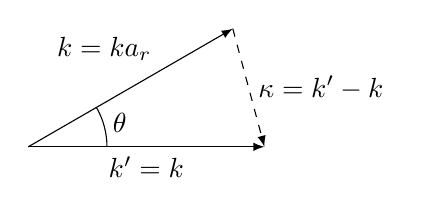
\begin{tikzpicture}
\draw[-latex] (0,0) -- (3,0) node[pos=0.5,below]{$\kvec{k}'=k\az$}coordinate(aa);
\draw[-latex] (0,0) --++ (30:3) node[pos=0.65,above left]{$\kvec{k}=k\kvec{a}_r$}coordinate(bb);
\draw[-latex,dashed] (bb)--(aa)node[pos=0.5,right]{$\kvec{\kappa}=\kvec{k}'-\kvec{k}$};
\draw([shift={(0:1)}]0,0) arc (0:30:1)node[pos=0.6,right]{$\theta$};
\end{tikzpicture}
\caption{بارن تخمین میں دو تفاعل موج: \عددی{\kvec{k}'} آمدی رخ جبکہ \عددی{\kvec{k}} بکھراو رخ ہے۔}
\label{شکل_بکھراو_آمدی_بکھراو_رخ}
\end{figure}


%=========
\ابتدا{مثال}
\اصطلاح{کم توانائی نرم کرہ بکھراو}۔\فرہنگ{بکھراو!کم توانائی نرم کرہ}\حاشیہب{low-energy soft-sphere scattering}\فرہنگ{scattering!low-energy soft-sphere} درج ذیل مخفیہ لیں۔ \حاشیہد{آپ سخت کرہ بکھراو \عددی{(V_0=\infty)} پر بارن تخمین کا اطلاق نہیں کر سکتے، چونکہ تکمل بے قابو بڑھتا ہے۔ آپ کو یاد رکھنا ہو گا کہ ہم مخفیہ کو کم زور تصور کرتے ہیں، جو خطہ بکھراو میں تفاعل موج کو تبدیل نہیں کرتا۔ تاہم سخت کرہ اس کو \عددی{Ae^{ikz}} سے\ترچھا{ صفر} کرتا ہے،جو بہت بڑی تبدیل ہے۔}
\begin{align}
	V(\kvec{r})=
	\begin{cases}
		V_0, & r\leq a \\
		0, & r>a 
	\end{cases}
\end{align}
کم توانائی بکھراو کی صورت میں (\عددی{\theta} اور \عددی{\phi} کا غیر تابع) حیطہ بکھراو
\begin{align}\label{مساوات_بکھراو_غیر_تابع_حیطہ_ہے}
	f(\theta, \phi)\cong-\frac{m}{2\pi\hslash^2}V_0\left(\frac{4}{3}\pi a^3\right)
\end{align}
ہے، تفریقی عمودی تراش 
\begin{align}
	\frac{\dif\sigma}{\dif\Omega}=\abs{f}^2\cong\left(\frac{2mV_0a^3}{3\hslash^2}\right)^2
\end{align}
اور کل عمودی تراش درج ذیل ہوگا۔ 
\begin{align}
	\sigma\cong4\pi\left(\frac{2mV_0a^3}{3\hslash^2}\right)^2
\end{align}
\انتہا{مثال}

\اصطلاح{کروی تشاکلی مخفیہ}\فرہنگ{کروی تشاکلی مخفیہ}\حاشیہب{spherical symmetrical potential}\فرہنگ{spherical symmetrical potential} \عددی{V(\kvec{r})=V(r)}کے لئے، جو ضروری نہیں کہ کم توانائی ہو، تخمین بارن سادہ روپ اختیار کرتا ہے۔ درج ذیل متعارف کرتے ہوئے 
\begin{align}
	\kvec{\kappa}\equiv \kvec{k}'-\kvec{k}
\end{align}
\عددی{\kvec{r}_0} تکمل کے قطبی محور کو \عددی{\kvec{\kappa}} پر رکھتے ہوئے
\begin{align}
	(\kvec{k}'-\kvec{k})\cdot \kvec{r}_0 = \kappa r_0\cos\theta_0
\end{align}
ہو گا۔ یوں
\begin{align}
	f(\theta)\cong-\frac{m}{2\pi\hslash^2}\int e^{i\kappa r_0\cos\theta_0}V(r_0)r^2_0\sin\theta_0\dif r_0\dif\theta_0\dif\phi_0
\end{align}
ہو گا۔ متغیر \عددی{\phi_0} کے لحاظ سے تکمل \عددی{2\pi} دیگا، اور \عددی{\theta_0} تکمل کو ہم پہلے دیکھ چکے ہیں (مساوات \حوالہ{مساوات_بکھراو_تھیٹا_تکمل} دیکھیں)۔ یوں \عددی{r} کے زیرنوشت کو نہ لکھتے ہوئے درج ذیل رہ جاتا ہے۔
\begin{align}
	f(\theta)\cong-\frac{2m}{\hslash^2\kappa}\int_{0}^{\infty}rV(r)\sin(\kappa r)\dif r، && \text{\small\RL{(کروی تشاکل)}}
\end{align}
\عددی{f} کی زاویائی تابعیت \عددی{\kappa} میں سموئی گئی ہے; شکل \حوالہ{شکل_بکھراو_آمدی_بکھراو_رخ} کو دیکھ کر درج ذیل لکھا جا سکتا ہے۔
\begin{align}\label{مساوات_بکھراو_کاپا}
	\kappa = 2k\sin(\theta/2)
\end{align}
\ابتدا{مثال}
\اصطلاح{یوکاوا بکھراو۔}\فرہنگ{بکھراو!یوکاوا}\حاشیہب{Yukawa scattering}\فرہنگ{scattering!Yukawa} \اصطلاح{یوکاوا مخفیہ}\فرہنگ{یوکاوا مخفیہ}\حاشیہب{Yukawa potential}\فرہنگ{Yukawa potential} ( جو جوہری مرکزہ کے اندر بندشی قوت کا ایک سادہ نمونہ پیش کرتا ہے) کا روپ درج ذیل ہے، جہاں \عددی{\beta} اور \عددی{\mu} مستقلات ہیں۔
\begin{align}
	V(r) = \beta\frac{e^{-\mu r}}{r}
\end{align}
تخمین بارن درج ذیل دیگا۔
\begin{align}\label{مساوات_بکھراو_اس_کو_حل_کرنا_ہو_گا}
	f(\theta)\cong-\frac{2m\beta}{\hslash^2\kappa}\int_{0}^{\infty}e^{-\mu r}\sin(\kappa r)\dif r=-\frac{2m\beta}{\hslash^2(\mu^2+\kappa^2)}
\end{align}
(آپ کو سوال \حوالہ{سوال_بکھراو_تکمل_حل_کریں} میں یہ تکمل حل کرنے کو کہا گیا ہے۔)
\انتہا{مثال}
\ابتدا{مثال}
\اصطلاح{ردرفورڈ بکھراو۔}\فرہنگ{بکھراو!ردرفورڈ}\حاشیہب{Rutherford scattering}\فرہنگ{scattering!Rutherford} مخفیہ یوکاوا میں \عددی{\beta=q_1q_2/4\pi\epsilon_0} اور \عددی{\mu=0} پُر کرنے سے مخفیہ کولمب حاصل ہوتا ہے، جو دو نقطی بار کے برقی باہم عمل کو بیان کرتا ہے۔ ظاہر ہے کہ حیطہ بکھراو
\begin{align}
	f(\theta)\cong-\frac{2mq_1q_2}{4\pi\epsilon_0\hslash^2\kappa^2}
\end{align}
ہو گا یا ( مساوات \حوالہ{مساوات_بکھراو_کاپا} اور مساوات \حوالہ{مساوات_بکھراو_ہلم_ہولٹز_طرز} استعمال کرتے ہوئے ) 
\begin{align}
	f(\theta)\cong-\frac{q_1q_2}{16\pi\epsilon_0E\sin^2(\theta/2)}
\end{align}
ہو گا۔ اس کا مربع ہمیں تفریقی عمودی تراش 
\begin{align}
	\frac{\dif\sigma}{\dif\Omega}=\left[\frac{q_1q_2}{16\pi\epsilon_0E\sin^2(\theta/2)}\right]^2
\end{align}
دیگا، جو ٹھیک کلیہ ردرفورڈ ( مساوات \حوالہ{مساوات_بکھراو_تفریقی_بکھراو_عمودی_تراش}) ہے۔ آپ دیکھ سکتے ہیں کہ کولمب مخفیہ کے لئے کلاسیکی میکانیات، تخمین بارن، اور کوانٹائی نظریہ میدان ایک جیسا نتیجہ دیتے ہیں۔ ہم کہہ سکتے ہیں کہ کلیہ ردرفورڈ نہایت \قول{مضبوط} کلیہ ہے۔
\انتہا{مثال}
\ابتدا{سوال}
اختیاری توانائی کے لئے، بارن تخمین میں، نرم کرہ بکھراو کا حیطہ بکھراو حاصل کریں۔ دکھائیں کہ کم توانائی حد میں اس کی تخفیف مساوات \حوالہ{مساوات_بکھراو_غیر_تابع_حیطہ_ہے} میں ہوگی۔
\انتہا{سوال}
\ابتدا{سوال}\شناخت{سوال_بکھراو_تکمل_حل_کریں}
مساوات \حوالہ{مساوات_بکھراو_اس_کو_حل_کرنا_ہو_گا} میں تکمل کی قیمت تلاش کر کے، دائیں ہاتھ کے ریاضی فقرے کی تصدیق کریں۔
\انتہا{سوال}
\ابتدا{سوال}
بارن تخمین میں، یوکاوا مخفیہ سے بکھراو کا کل عمودی تراش تلاش کریں۔ اپنے جواب کو \عددی{E} کا تفاعل لکھیں۔
\انتہا{سوال}
\ابتدا{سوال}
درج ذیل اقدام سوال \حوالہ{سوال_بکھراو_کم_توانائی_کروی_ڈلٹا} کے مخفیہ کے لئے کریں۔
\begin{enumerate}[a.]
\item
 کم توانائی تخمین بارن میں \عددی{f(\theta)}، \عددی{D(\theta)}، اور \عددی{\sigma} کا حساب لگائیں۔
\item
 تخمین بارن میں اختیاری توانائیوں کے لئے \عددی{f(\theta)} کا حساب لگائیں۔
\item
دکھائیں کہ آپ کے نتائج مناسب طریق میں سوال \حوالہ{سوال_بکھراو_کم_توانائی_کروی_ڈلٹا} کے جواب کے مطابق ہیں۔
\end{enumerate}
\انتہا{سوال}

%=================================

\جزوحصہ{تسلسل بارن}
تخمین بارن روح کے لحاظ سے کلاسیکی نظریہ بکھراو میں \اصطلاح{تخمین ضرب}\فرہنگ{تخمین!ضرب}\حاشیہب{impulse approximation}\فرہنگ{approximation!impulse} کی طرح ہے۔ ایک ذرے کو منتقل عرضی ضرب کا حساب کرنے کے لئے ہم تخمین ضرب میں فرض کرتے ہیں
 کہ ذرہ سیدھی لیکر پر حرکت کیے جاتا ہے (شکل \حوالہ{شکل_بکھراو_تخمین_ضرب})۔ ایسی صورت میں درج ذیل ہوگا۔
\begin{align}
	I=\int F_\perp\dif t&&\text{\small\RL{(عرضی ضرب)}}
\end{align}
%
\begin{figure}
\centering
\begin{tikzpicture}
\pgfmathsetmacro{\ang}{atan(1/2.5)}
\draw[] (0,0) -- (6,0) node[pos=0.55, circle, inner sep=1.5pt,fill=black]{} node[pos=0.55, below]{\RL{نقطہ بکھراو}} ;
\draw[dashed] (0,1) -- (6,1) node[pos=0.5, circle, inner sep=1.5pt,fill=black]{};
\draw[thick,-stealth] (0,1) to [out=0,in=-160] (6,2) node[above]{\RL{اصل خط حرکت}};
\draw[-stealth] (3,1) -- (3,2) node[above]{$F_{\perp}$}; 
\draw[dashed] (3.5,1) -- (6,2);
\draw[] ([shift={(0:1)}]3.5,1) arc (0:\ang:1) node[pos=0.6,right]{$\theta$};
\draw[stealth-stealth] (0.25,0) --++ (0,1) node[pos=0.5,left]{$b$};
\end{tikzpicture}
\caption{ ذرہ کے منتقل معیار حرکت کا حساب کرتے ہوئے،تخمین ضرب کی ترکیب میں فرض کیا جاتا ہے کہ ذرہ بغیر مڑے سیدھی لکیر پر حرکت کیے جاتا ہے۔}
\label{شکل_بکھراو_تخمین_ضرب}
\end{figure}
اگر ذرہ زیادہ نہیں مڑے، تب ذرے کو منتقل معیار حرکت کی یہ ایک اچھی تخمین ہوگی، اور یوں زاویہ بکھراو درج ذیل ہوگا، جہاں \عددی{p} آمدی معیار حرکت ہے۔
\begin{align}
	\theta\cong\tan^{-1}(I/p)
\end{align}
اسے ہم \قول{ رتبہ اول} تخمین ضرب کہہ سکتے ہیں (ابتدائی، نہ مڑنے کی، صورت کو صفر رتبی کہیں گے)۔ اسی طرح، صفر رتبی تخمین بارن میں آمدی مستوی موج بغیر تبدیلی کے گزرے گی، اور ہم نے جو کچھ گزشتہ حصہ میں دیکھا در حقیقت اس کی اول رتبی تصحیح ہے۔ اسی تصور کو بار بار استعمال کر کے زیادہ بلند رتبی تصحیح کا تسلسل پیدا کیا جا سکتا ہے، اور توقع کی جا سکتی ہے کہ یہ بالکل ٹھیک جواب پر مرکوز ہو گا۔

مساوات شروڈنگر کا تکملی روپ 
\begin{align}
	\psi(\kvec{r})=\psi_0(\kvec{r})+\int g(\kvec{r}-\kvec{r}_0)V(\kvec{r}_0)\psi(\kvec{r}_0)\dif^{\,3}\kvec{r}_0
\end{align}
لکھا جا سکتا ہے، جہاں \عددی{\psi_0} آمدی موج ہے،
\begin{align}
	g(\kvec{r})\equiv-\frac{m}{2\pi\hslash^2}\frac{e^{ikr}}{r}
\end{align}
تفاعل گرین ( جس میں میں نے اپنی آسانی کے لئے جزو ضربی \عددی{2m/\hslash^2} شامل کیا ہے)، اور \عددی{V} مخفیہ بکھراو ہے۔درج ذیل (سادہ روپ) لکھا جا سکتا ہے۔
\begin{align}
	\psi = \psi_0+\int gV\psi
\end{align}
فرض کریں ہم \عددی{\psi} کی اس ریاضی جملے کو لیکر ا تکمل کی علامت کے اندر لکھیں۔
\begin{align}
	\psi=\psi_0+\int gV\psi_0+\iint gVgV\psi
\end{align}
اس عمل کو بار بار دہرانے سے ہمیں \عددی{\psi} کا تسلسل:
\begin{align}\label{مساوات_بکھراو_بارن_تخمین_تسلسل}
	\psi=\psi_0+\int gV\psi_0+\iint gVgV\psi_0+\iiint gVgVgV\psi_0+\dots
\end{align}
 حاصل ہوگا۔ ہر متکمل میں صرف \ترچھا{آمدی} تفاعل موج \عددی{\psi_0}، اور اس کے علاوہ \عددی{gV} کے مزید زیادہ طاقتیں پائی جاتی ہیں۔ بارن کی تخمین اول اس تسلسل کو دوسرے جزو کے بعد ختم کرتی ہے، لیکن آپ دیکھ سکتے ہیں کہ بلند رتبی تصحیح کس طرح پیدا کی جائیں گی۔
\begin{figure}
\centering
\begin{tikzpicture}
\pgfmathsetmacro{\a}{1.25}
\pgfmathsetmacro{\r}{0.75}
\pgfmathsetmacro{\d}{0.25}
\draw[->-=0.6] (0,0) node[left]{$\psi=$} --++ (\a,0) node[pos=0.5,below]{$\psi_0$};
\draw[] (\a +\d,0) node[]{$+$};
\draw[->-=0.25] (\a+2*\d,0) --++ (\a,0) node[pos=0.25,below]{$\psi_0$} coordinate(aa);
\draw[] (aa) node[circle, inner sep= 1.5pt, fill=black]{} node[below]{$V$} circle (\r);
\draw[] (aa) --++ (30:1.25) node[pos=0.25,shift={(-60:0.5em)}]{$g$};
\draw[] (2*\a +4*\d+\r,0) node[]{$+$};
\draw[->-=0.3] (2*\a +5*\d+\r,0) --++ (\a,0) node[pos=0.3,below,xshift=-0.1em]{$\psi_0$} coordinate(aa);
\draw[] (aa) node[circle, inner sep= 1.5pt, fill=black]{} node[below]{$V$} circle (\r);
\draw[] (aa) --++ (20:0.5) node[pos=0.5,shift={(110:0.5em)}]{$g$} node[circle, inner sep=1.5pt,fill=black]{} node[below]{$V$} --++ (80:1) node[pos=0.5,right]{$g$};
\draw[] (3*\a +6*\d+2*\r,0) node[]{$+$};
\draw[->-=0.3] (3*\a +7*\d+2*\r,0) --++ (0.75*\a,0) node[pos=0.3,below,xshift=-0.1em]{$\psi_0$} node[circle, inner sep= 1.5pt, fill=black]{} node[above]{$V$}coordinate(bb); 
\draw[] (4*\a +7*\d+2*\r,0) coordinate(aa) circle (\r);
\draw[] (bb) --++ (-40:0.5) node[pos=0.5,shift={(-130:0.5em)}]{$g$} node[circle, inner sep=1.5pt,fill=black]{} node[below]{$V$} --++ (45:0.75) node[pos=0.5,shift={(-45:0.5em)}]{$g$}node[circle, inner sep=1.5pt,fill=black]{}node[above left]{$V$}--++(-10:1)node[pos=0.75,above]{$g$};
\draw[] (5*\a +7*\d+3*\r,0) node[]{$+\cdots$};
\end{tikzpicture}
\caption{بارن تسلسل (مساوات \حوالہ{مساوات_بکھراو_بارن_تخمین_تسلسل}) کی نظیری مفہوم۔}
\label{شکل_بکھراو_نظیری_مفہوم}
\end{figure}

بارن تسلسل کا خاکہ شکل \حوالہ{شکل_بکھراو_نظیری_مفہوم} میں پیش کیا گیا ہے۔ صفر رتبی \عددی{\psi} پر مخفیہ کا کوئی اثر نہیں ہوگا؛ اول رتبی میں اسے ایک \قول{چوٹ} پڑتی ہے، جس کے بعد یہ کسی نئے رخ چلتا ہے؛ دوم رتبی میں اسے ایک چوٹ پڑتی ہے جس کے بعد یہ ایک نئے مقام کو پہنچتا ہے جہاں اسے دوبارہ ایک چوٹ پڑتی ہے جس کے بعد یہ ایک نئی راہ پر چل نکلتا ہے، وغیرہ، وغیرہ۔ اسی بنا پر بعض اوقات تفاعل گرین کو \اصطلاح{اشاعت کار}\فرہنگ{اشاعت کار}\حاشیہب{propagator}\فرہنگ{propagator} کہا جاتا ہے؛ جو ایک باہم عمل سے دوسرے باہم عمل تک خلل کی اشاعت کے بارے میں بتاتا ہے۔ تسلسل بارن اضافیتی کوانٹائی میکانیات کی\اصطلاح{ فائن من تشریح}\فرہنگ{فائن من!تشریح}\حاشیہب{Feynman's formulation}\فرہنگ{Feynman!formulation} کا سبب بنا جس میں \اصطلاح{اشکال فائن من}\فرہنگ{فائن من!اشکال}\حاشیہب{Feynman diagram}\فرہنگ{Feynman!diagram} میں جزو ضربی راس \عددی{V} اور اشاعت کار \عددی{g} کو ایک ساتھ جوڑ کر سب کچھ بیان کیا جاتا ہے۔

\ابتدا{سوال}
تخمین ضرب میں ردرفورڈ بکھراو کے لئے \عددی{\theta} ( بطور ٹکراؤ مقدار معلوم کا تفاعل) تلاش کریں۔ دکھائیں کہ، مناسب حدوں کے اندر، آپ کا نتیجہ بالکل ٹھیک ریاضی فقرے (سوال \حوالہ{سوال_بکھراو_پہلا}-الف) کے مطابق ہے۔
\انتہا{سوال}
\ابتدا{سوال}
بارن کی دوسری تخمین میں کم توانائی نرم کرہ بکھراو کے لئے حیطہ بکھراو تلاش کریں۔

\ترچھا{جواب:} \عددی{-(2mV_0a^3/3\hslash^2)[1-(4mV_0a^2/5\hslash^2)]}
\انتہا{سوال}
\جزوحصہء{اضافی سوالات برائے باب \حوالہ{باب_بکھراو}}
\ابتدا{سوال}\شناخت{سوال_بکھراو_اضافی_پہلا}
یک بُعدی مساوات شروڈنگر کے لئے تفاعل گرین تلاش کر کے (مساوات \حوالہ{مساوات_بکھراو_دوبارہ_نظر} کا مماثل) تکملی روپ تیار کریں۔\ترچھا{جواب:}
\begin{align}
	\psi(x)=\psi_0(x)-\frac{im}{\hslash^2k}\int_{-\infty}^{\infty}e^{ik\abs{x-x_0}}V(x_0)\psi(x_0)\dif x_0
\end{align}
\انتہا{سوال}
\ابتدا{سوال}\شناخت{سوال_بکھراو_اضافی_دوم}
یک بُعدی بکھراو کے لئے سوال \حوالہ{سوال_بکھراو_اضافی_پہلا} کا نتیجہ استعمال کرتے ہوئے (مبدا پر بغیر \قول{ اینٹوں کی دیوار} کی صورت میں وقفہ \عددی{-\infty<x<\infty} پر ) تخمین بارن تیار کریں۔ یعنی \عددی{\psi_0(x)=Ae^{ikx}} منتخب کر کے، اور \عددی{\psi(x_0)\cong\psi_0(x_0)} تصور کرتے ہوئے، تکمل کی قیمت تلاش کریں۔ دکھائیں کہ انعکاسی عددی سر درج ذیل روپ اختیار کرتا ہے۔
\begin{align}
	R\cong\left(\frac{m}{\hslash^2k}\right)^2\abs{\int_{-\infty}^{\infty}e^{2ikx}V(x)\dif x}^2
\end{align}
\انتہا{سوال}
\ابتدا{سوال}
ایک ڈیلٹا تفاعل (مساوات \حوالہ{مساوات_شروڈنگر_کنواں_مخفیہ}) اور ایک متناہی چوکور کنواں (مساوات \حوالہ{مساوات_شروڈنگر_متناہی_چکور_کنواں_مخفیہ}) سے بکھراو کے لئے ترسیلی عددی سر \عددی{(T = 1 - R)} کو یک بُعدی تخمین بارن (سوال \حوالہ{سوال_بکھراو_اضافی_دوم}) سے حاصل کریں۔ اپنے جوابات کا موازنہ ٹھیک جوابات ( مساوات \حوالہ{مساوات_شروڈنگر_انعکاس_ترسیل_مستقل} اور مساوات \حوالہ{مساوات_شروڈنگر_ترسیلی_حل}) کے ساتھ کریں۔
\انتہا{سوال}
\ابتدا{سوال}
آگے رخ حیطہ بکھراو کے خیالی جزو اور کل عمودی تراش کے بیچ رشتہ پیش کرنے والا \اصطلاح{مسئلہ بصریات:}\فرہنگ{مسئلہ!بصریات}\حاشیہب{optical theorem}\فرہنگ{theorem!optical} 
\begin{align}
	\sigma = \frac{4\pi}{k}Im(f(0))
\end{align}
ثابت کریں۔ \ترچھا{اشارہ:} مساوات \حوالہ{مساوات_بکھراو_درکار_آخری_الف} اور مساوات \حوالہ{مساوات_بکھراو_درکار_آخری_ب} استعمال کریں۔
\انتہا{سوال}
